\documentclass[11pt]{article} % ~~~~~~~~~~~~~~~~~~~~~~~ %
%														%
\usepackage{etex}													%
\usepackage[english]{babel}											%
\usepackage[a4paper,margin=3cm]{geometry}							%
\usepackage{dsfont}													%
\usepackage{booktabs}												%
\usepackage{array}													%
\usepackage{bm}														%
\usepackage{enumerate}												%
\usepackage[table]{xcolor}											%
\usepackage{amsmath,amssymb,amsfonts}								% 
\usepackage{multirow}												%
\usepackage{graphicx}												% 
\DeclareGraphicsExtensions{.pdf,.png,.jpg,.mps}						%
\usepackage[colorlinks=true,linkcolor=black!90!white]{hyperref}		%
\usepackage{framed}													%
\usepackage[amsmath,thmmarks,framed,hyperref]{ntheorem}				%
\usepackage{pdftexcmds}												%
\usepackage{eso-pic}												%
\usepackage[switch, pagewise, mathlines]{lineno}					%
\usepackage[color=red!20!white, textwidth=5cm]{todonotes}			%
\usepackage{algorithm}												%
\usepackage[noend]{algpseudocode}									%
\usepackage{acronym}												%
\usepackage{subcaption}												%
\usepackage{url}													%
\usepackage{bm}														%
\usepackage{tikz}				% (note: AFTER \pdfminorversion)	%
\usepackage{pgfplots}												%
\let\labelindent\relax												%
\usepackage{enumitem}												%
\everymath={\displaystyle}											%
% ~~~~~~~~~~~~~~~~~~~~~~~~~~~~~~~~~~~~~~~~~~~~~~~~~~~~~~~~~~~~~~~~~ %

								%
% --> numbered environments style ridefinition example:
%
%\newtheoremstyle{mystyle}	% name of the style
%{3pt}						% vertical space before the environment
%{8pt}						% vertical space after the environment
%{}							% body's font
%{}							% indentation (empty -> \parindent)
%{\bfseries}				% header's font
%{.}						% punctuation after the header
%{\newline}					% space after the header (empty -> \newline)
%{\thmname{#1}\thmnumber{ #2}\thmnote{ #3}}	% header formatting
%											% (cancel for the default)
%
%
% --> numbered environments ridefinition example
%
% \newtheorem	{unique_name}			% environment's ID
%										% (use \begin{unique_name})
%				[associated_counter]	% [optional] could be not
%										% unambiguous
%				{text}					% what will be printed
%				[section]				% [optional] to which kind of
%										% sectioning the enumeration
%										% will be tied



\theoremstyle		{nonumberplain}
\def\theoremframecommand{\colorbox[rgb]{0.95,0.95,0.95}}
\newshadedtheorem	{instructions}		{Instructions:}

							%
% in order to call \includegraphics{myImage} instead of \includegraphics{../images/myImage}
\graphicspath{{../Images/}}

\pgfdeclarelayer{ultrabackground}
\pgfdeclarelayer{background}
\pgfdeclarelayer{foreground}
\pgfsetlayers{ultrabackground,background,main,foreground}


% \begin{pgfonlayer}{foreground}
% 	%
% 	%
% \end{pgfonlayer}

				%
\def\TablesRowsColor{black!8}
\def\TablesColumnsColor{black!4}

\newcolumntype
{g}
{
	>{\centering \columncolor{\TablesColumnsColor} \arraybackslash}
	p{0.15\textwidth}
	<{}
}

\newcolumntype
{w}
{
	>{\centering \arraybackslash}
	p{0.15\textwidth}
	<{}
}

				%
\newcommand{\source}[1]
{
	\ifthenelse
	{\boolean{writefilenames}}
	{
		\begin{center}
		{\color[rgb]{0.6,0.6,0.6} \rule{\columnwidth}{0.2mm}}
		$\downarrow\;\;$ \textbf{#1} $\;\;\downarrow$
		\end{center}
	}
	{}
}


\newcommand{\EstimatedSignal}						[0]	{\widehat{\Signal}}
\newcommand{\OptimallyEstimatedSignal}				[0]	{\widehat{\Signal}^{*}}
\newcommand{\OptimallyBayesEstimatedSignal}			[0]	{\widehat{\Signal}^{*}_{\text{Bayes}}}
\newcommand{\OptimallyCostFunctionEstimatedSignal}	[0]	{\widehat{\Signal}^{*}_{\text{c.f.}}}
%
\newcommand{\EstimatedSignalAt}						[1]	{\EstimatedSignal \left( #1 \right)}
\newcommand{\OptimallyEstimatedSignalAt}			[1]	{\OptimallyEstimatedSignal \left( #1 \right)}
\newcommand{\OptimallyBayesEstimatedSignalAt}		[1]	{\OptimallyBayesEstimatedSignal \left( #1 \right)}
\newcommand{\OptimallyCostFunctionEstimatedSignalAt}[1]	{\OptimallyCostFunctionEstimatedSignal \left( #1 \right)}
%
\newcommand{\EstimatedSignalAtSet}						[1]	{\EstimatedSignal_{#1}}
\newcommand{\OptimallyEstimatedSignalAtSet}				[1]	{\OptimallyEstimatedSignal_{#1}}
\newcommand{\OptimallyBayesEstimatedSignalAtSet}		[1]	{\OptimallyBayesEstimatedSignal_{#1}}
\newcommand{\OptimallyCostFunctionEstimatedSignalAtSet}	[1]	{\OptimallyCostFunctionEstimatedSignal_{#1}}




\newcommand{\EstimatedEigenfunctionWeight}			[1]
			{\widehat{a}_{#1}}
\newcommand{\SetOfEstimatedEigenfunctionsWeights}	[0]
			{\widehat{\SetOfEigenfunctionsWeights}}
\newcommand{\EigenfunctionsWeightsEstimationError}	[0]
			{\widetilde{\SetOfEigenfunctionsWeights}}




\newcommand{\EstimatedEigenfunctionWeightOfSensor}			[2]
			{\widehat{a}_{#1, #2}}
\newcommand{\SetOfEstimatedEigenfunctionsWeightsOfSensor}	[1]
			{\widehat{\SetOfEigenfunctionsWeights}_{#1}}
\newcommand{\EigenfunctionsWeightsEstimationErrorOfSensor}	[1]
			{\widetilde{\SetOfEigenfunctionsWeights}_{#1}}
\newcommand{\LocallyEstimatedEigenfunctionWeightOfSensor}	[2]
			{\widehat{a}_{#1, #2}^{loc}}




\newcommand{\SetOfLocallyEstimatedEigenfunctionsWeights}				[0]
			{\widehat{\SetOfEigenfunctionsWeights}^{\text{loc}}}
\newcommand{\SetOfLocallyEstimatedEigenfunctionsWeightsOfSensor}		[1]
			{\widehat{\SetOfEigenfunctionsWeights}^{\text{loc}}_{#1}}
\newcommand{\SetOfLocallyBayesEstimatedEigenfunctionsWeights}			[0]
			{\widehat{\SetOfEigenfunctionsWeights}_{\text{Bayes}}^{\text{loc}}}
\newcommand{\SetOfLocallyCostFunctionEstimatedEigenfunctionsWeights}	[0]
			{\widehat{\SetOfEigenfunctionsWeights}_{\text{c.f.}}^{\text{loc}}}
%
\newcommand{\SetOfLocallyBayesEstimatedEigenfunctionsWeightsOfSensor}			[1]
			{\widehat{\SetOfEigenfunctionsWeights}_{\text{Bayes}, #1}^{\text{loc}}}
\newcommand{\SetOfLocallyCostFunctionEstimatedEigenfunctionsWeightsOfSensor}	[1]
			{\widehat{\SetOfEigenfunctionsWeights}_{\text{c.f.}, #1}^{\text{loc}}}
%
%
\newcommand{\SetOfCentrallyEstimatedEigenfunctionsWeights}				[0]
			{\widehat{\SetOfEigenfunctionsWeights}^{\text{cen}}}
\newcommand{\SetOfCentrallyBayesEstimatedEigenfunctionsWeights}			[0]
			{\widehat{\SetOfEigenfunctionsWeights}_{\text{Bayes}}^{\text{cen}}}
\newcommand{\SetOfCentrallyCostFunctionEstimatedEigenfunctionsWeights}	[0]
			{\widehat{\SetOfEigenfunctionsWeights}_{\text{c.f.}}^{\text{cen}}}
%
\newcommand{\SetOfCentrallyBayesEstimatedEigenfunctionsWeightsOfSensor}			[1]
			{\widehat{\SetOfEigenfunctionsWeights}_{\text{Bayes}, #1}^{\text{cen}}}
\newcommand{\SetOfCentrallyCostFunctionEstimatedEigenfunctionsWeightsOfSensor}	[1]
			{\widehat{\SetOfEigenfunctionsWeights}_{\text{c.f.}, #1}^{\text{cen}}}
%
%
\newcommand{\SetOfDistributelyEstimatedEigenfunctionsWeights}				[0]
			{\widehat{\SetOfEigenfunctionsWeights}^{\text{dis}}}
\newcommand{\SetOfDistributelyBayesEstimatedEigenfunctionsWeights}			[0]
			{\widehat{\SetOfEigenfunctionsWeights}_{\text{Bayes}}^{\text{dis}}}
\newcommand{\SetOfDistributelyCostFunctionEstimatedEigenfunctionsWeights}	[0]
			{\widehat{\SetOfEigenfunctionsWeights}_{\text{c.f.}}^{\text{dis}}}
%
\newcommand{\SetOfDistributelyBayesEstimatedEigenfunctionsWeightsOfSensor}			[1]
			{\widehat{\SetOfEigenfunctionsWeights}_{\text{Bayes}, #1}^{\text{dis}}}
\newcommand{\SetOfDistributelyCostFunctionEstimatedEigenfunctionsWeightsOfSensor}	[1]
			{\widehat{\SetOfEigenfunctionsWeights}_{\text{c.f.}, #1}^{\text{dis}}}




\newcommand{\MaxAdmittableDistanceBtwOptimalCentralizedAndSuboptimalDistributedEstimates}	[0]
			{d_{\text{o.c.}-\text{s.d.}}^{\text{max}}}



\newcommand{\DistanceBtwLocalApproximatedBayesAndLocalApproximatedCostFunction}	[0]
	{d_{\text{l.a.B. - l.a.c.f.}}}
\newcommand{\DistanceBtwLocalOptimalBayesAndLocalApproximatedCostFunction}		[0]
	{d_{\text{l.o.B. - l.a.c.f.}}}
\newcommand{\DistanceBtwLocalOptimalBayesAndLocalApproximatedBayes}				[0]
	{d_{\text{l.o.B. - l.a.B.}}}



\newcommand{\NaiveDistributedEstimatorOfEigenfunctionsWeights}		[0]
	{\widehat{\SetOfEigenfunctionsWeights}_{\text{dis}}^{\text{naive}}}
%
\newcommand{\GuessedDistributedEstimatorOfEigenfunctionsWeights}	[0]
	{\widehat{\SetOfEigenfunctionsWeights}_{\text{dis}}^{\text{guess}}}
\newcommand{\GuessedDistributedEstimatorOfEigenfunctionsWeightsOfGuess}	[1]
	{\GuessedDistributedEstimatorOfEigenfunctionsWeights \left( #1 \right)}




\newcommand{\DefinedAs}			[0]	{\mathrel{\mathop:}=}
\newcommand{\IDefinedAs}		[0]	{=\mathrel{\mathop:}}
%\newcommand{\DefinedAs}			[0]	{\mathrel{\doteq}}
%\newcommand{\IDefinedAs}		[0]	{\mathrel{\doteq}}


\newcommand{\ExponentialOf}		[1]	{\mathrm{exp} \left( #1 \right)}
\newcommand{\LogarithmOf}		[1]	{\mathrm{ln} \left( #1 \right)}
\newcommand{\ConvexHullOf}		[1]	{\mathcal{H}_{\textrm{cvx}} \left( #1 \right)}
\newcommand{\ConicalHullOf}		[1]	{\mathcal{H}_{\textrm{cnc}} \left( #1 \right)}
\newcommand{\BoundaryOf}		[1]	{\mathcal{B} \left( #1 \right)}
\newcommand{\InteriorOf}		[1]	{\mathrm{int} \left( #1 \right)}
\newcommand{\MeasureOfIn}		[2]	{\mu_{#2} \left( #1 \right)}


\newcommand{\MaximumOfOne}		[1]	{\mathrm{max} \left\lbrace #1 \right\rbrace}
\newcommand{\MaximumOfTwo}		[2]	{\mathrm{max} \left\lbrace #1, #2 \right\rbrace)}
\newcommand{\MaximumOfThree}	[3]	{\mathrm{max} \left\lbrace #1, #2, #3 \right\rbrace)}
\newcommand{\MinimumOfOne}		[1]	{\mathrm{min} \left\lbrace #1 \right\rbrace}
\newcommand{\MinimumOfTwo}		[2]	{\mathrm{min} \left\lbrace #1, #2 \right\rbrace)}
\newcommand{\MinimumOfThree}	[3]	{\mathrm{min} \left\lbrace #1, #2, #3 \right\rbrace)}


\newcommand{\CostFunction}				[0]	{Q}
\newcommand{\CostFunctionOf}			[1]	{\CostFunction \left( #1 \right)}
\newcommand{\CostFunctionOfSensor}		[1]	{\CostFunction_{#1}}
\newcommand{\CostFunctionOfSensorOf}	[2]	{\CostFunctionOfSensor{#1} \left( #2 \right)}


\newcommand{\KroneckerDeltaOf}			[2]	{\delta_{#1 #2}}


\newcommand{\FloorOf}			[1]	{\lfloor #1 \rfloor}
\newcommand{\CeilOf}			[1]	{\lceil #1 \rceil}
\newcommand{\SaturationOf}		[1]	{\mathrm{sat} \left( #1 \right)}
\newcommand{\PositivePartOf}	[1]	{\left[ #1 \right]_{+}}
\newcommand{\NegativePartOf}	[1]	{\left[ #1 \right]_{-}}


\newcommand{\GammaFunctionOf}	[1]	{\Gamma \left( #1 \right)}
\newcommand{\BetaFunctionOf}	[2]	{B \left( #1, #2 \right)}


\newcommand{\CholeskyFactorOf}	[1]	{\mathrm{chol} \left( #1 \right)}


\newcommand{\BigOOf}			[1]	{O \left( #1 \right)}
\newcommand{\SmallOOf}			[1]	{o \left( #1 \right)}


\newcommand{\PochhammerOf}		[2]	{\left( #1 \right)_{#2}}


\DeclareMathOperator*{\argmax}{arg\,max}
\DeclareMathOperator*{\argmin}{arg\,min}

\newcommand{\SensorIndex}			{s}
\newcommand{\SensorIndexTwo}		{r}
\newcommand{\SensorIndexThree}		{q}
%
\newcommand{\MeasurementIndex}		{m}
\newcommand{\MeasurementIndexTwo}	{n}
\newcommand{\MeasurementIndexThree}	{p}
%
\newcommand{\TimeIndex}				{t}
\newcommand{\TimeIndexTwo}			{\tau}
\newcommand{\TimeIndexThree}		{\tau'}
%
\newcommand{\EigenvalueIndex}		{k}
\newcommand{\EigenvalueIndexTwo}	{i}
\newcommand{\EigenvalueIndexThree}	{g}
%
\newcommand{\EigenvectorIndex}		{\EigenvalueIndex}
\newcommand{\EigenvectorIndexTwo}	{\EigenvalueIndexTwo}
\newcommand{\EigenvectorIndexThree}	{\EigenvalueIndexThree}
%
\newcommand{\EigenfunctionIndex}		{\EigenvalueIndex}
\newcommand{\EigenfunctionIndexTwo}		{\EigenvalueIndexTwo}
\newcommand{\EigenfunctionIndexThree}	{\EigenvalueIndexThree}



\newcommand{\NumberOfEigenvalues}					[0]	{E}
\newcommand{\NumberOfEigenvectors}					[0]	{\NumberOfEigenvalues}
\newcommand{\NumberOfEigenfunctions}				[0]	{\NumberOfEigenvalues}
\newcommand{\NumberOfSensors}						[0]	{S}
\newcommand{\NumberOfMeasurements}					[0]	{M}
\newcommand{\NumberOfMeasurementsOfSensor}			[1]	{\NumberOfMeasurements_{#1}}
\newcommand{\NumberOfMeasurementsOfAuxiliaryGrid}	[0]	{\NumberOfMeasurements_{G}}
\newcommand{\NumberOfInputLocations}				[0]	{\NumberOfMeasurements}
\newcommand{\NumberOfInputLocationsOfSensor}		[1]	{\NumberOfMeasurements_{#1}}
\newcommand{\NumberOfInputLocationsOfAuxiliaryGrid}	[0]	{\NumberOfMeasurements_{G}}
\newcommand{\NumberOfTimeIndexes}					[0]	{T}



\newcommand{\DimensionOfInputLocationsDomain}		[0]	{D}
\newcommand{\IdentityMatrix}		[1]	{I_{#1}}
\newcommand{\DiagonalMatrixOf}		[1]	{\mathrm{diag} \left( #1 \right)}
\newcommand{\OnesVector}			[0]	{\mathds{1}}

\newcommand{\TraceOf}				[1]	{\mathrm{tr} \left( #1 \right)}
\newcommand{\DeterminantOf}			[1]	{\mathrm{det} \left( #1 \right)}

\newcommand{\Eigenvalue}			[0]	{\lambda}
\newcommand{\EigenvalueOfIndex}		[1]	{\Eigenvalue_{#1}}
\newcommand{\MaximalEigenvalue}		[0]	{\Eigenvalue_{\mathrm{max}}}
\newcommand{\MinimalEigenvalue}		[0]	{\Eigenvalue_{\mathrm{min}}}
\newcommand{\SetOfEigenvaluesOf}	[1]	{\mathrm{eig} \left( #1 \right)}

\newcommand{\Eigenvector}			[0]	{v}
\newcommand{\EigenvectorOfIndex}	[1]	{\Eigenvector_{#1}}

\newcommand{\SpectralRadius}		[0]	{\mu}
\newcommand{\SpectralRadiusOf}		[1]	{\SpectralRadius \left( #1 \right)}

\newcommand{\KernelOf}				[1]	{\mathrm{Ker} \left( #1 \right)}
\newcommand{\SpanOf}				[1]	{\mathrm{span} \left\langle #1 \right\rangle}

\newcommand{\VectorizationOf}		[1] {\mathrm{vec} \left( #1 \right)}
\newcommand{\HalfVectorizationOf}	[1] {\mathrm{vech} \left( #1 \right)}
\newcommand{\MatricizationOf}		[1] {\mathrm{mat} \left( #1 \right)}
\newcommand{\HalfMatricizationOf}	[1] {\mathrm{math} \left( #1 \right)}


\newcommand{\GaussianDistribution}					[2]	{\mathcal{N} \left( #1, #2 \right)}
\newcommand{\GammaDistribution}						[2]	{\mathrm{Gamma} \left( #1, #2 \right)}
\newcommand{\InverseGammaDistribution}				[2]	{\mathrm{Inv-Gamma} \left( #1, #2 \right)}
\newcommand{\ChiSquareDistribution}					[0]	{\chi^{2}}
\newcommand{\ChiSquareDistributionOfIndex}			[1]	{\ChiSquareDistribution \left( #1 \right)}
\newcommand{\InverseChiSquareDistribution}			[0]	{\mathrm{Inv-}\chi^{2}}
\newcommand{\InverseChiSquareDistributionOfIndex}	[1]	{\InverseChiSquareDistribution \left( #1 \right)}
\newcommand{\UniformDistribution}					[2]	{\mathcal{U} \left[ #1, #2 \right]}
\newcommand{\ExponentialDistribution}				[1]	{\mathrm{Exp} \left( #1 \right)}
\newcommand{\BernoulliDistribution}					[1]	{\mathcal{B} \left( #1 \right)}
\newcommand{\BinomialDistribution}					[2]	{\mathrm{Bin} \left( #1, #2 \right)}


\newcommand{\SetOfComplexNumbers}					[0]	{\mathbb{C}}
\newcommand{\SetOfRealNumbers}						[0]	{\mathbb{R}}
\newcommand{\SetOfRealPositiveNumbers}				[0]	{\mathbb{R}_{+}}
\newcommand{\SetOfRationalNumbers}					[0]	{\mathbb{Q}}
\newcommand{\SetOfRationalPositiveNumbers}			[0]	{\mathbb{Q}_{+}}
\newcommand{\SetOfNaturalNumbers}					[0]	{\mathbb{N}}
\newcommand{\SetOfNaturalPositiveNumbers}			[0]	{\mathbb{N}_{+}}

\newcommand{\SetOfSquareSummableInfiniteVectors}			[0]	{\ell}
\newcommand{\SetOfWeightedSquareSummableInfiniteVectors}	[0]	{\textsl{l}_{\RKHS}}
\newcommand{\SetOfSquareIntegrableFunctions}				[0]	{\textsl{L}^{2}}
\newcommand{\SetOfSquareIntegrableFunctionsIn}				[1]	{\textsl{L}^{2} \left( #1 \right)}

\newcommand{\Signal}							[0]	{f}
\newcommand{\SignalOne}							[0]	{f}
\newcommand{\SignalTwo}							[0]	{g}
\newcommand{\SignalAt}							[1]	{\Signal \left( #1 \right)}
\newcommand{\SignalOneAt}						[1]	{\SignalOne \left( #1 \right)}
\newcommand{\SignalTwoAt}						[1]	{\SignalTwo \left( #1 \right)}



\newcommand{\StochasticProcess}					[0]	{\mathcal{F}}
\newcommand{\StochasticProcessRealization}		[0]	{\textsl{f}}
\newcommand{\StochasticProcessAt}				[1]	{\StochasticProcess \left( #1 \right)}
\newcommand{\StochasticProcessRealizationAt}	[1]	{\StochasticProcessRealization \left( #1 \right)}



\newcommand{\InfiniteVector}				[0]	{\mathbf{v}}
\newcommand{\InfiniteVectorOne}				[0]	{\mathbf{v}}
\newcommand{\InfiniteVectorTwo}				[0]	{\mathbf{w}}



\newcommand{\InputLocationsDomain}			[0] {\mathcal{D}}
\newcommand{\InputLocationsDomainOfSensor}	[1] {\InputLocationsDomain_{#1}}
\newcommand{\MeasurementsDomain}			[0] {\mathcal{M}}
\newcommand{\MeasurementsDomainOfSensor}	[1] {\MeasurementsDomain_{#1}}



\newcommand{\InputLocation}							[0]	{x}
\newcommand{\InputLocationOne}						[0]	{x}
\newcommand{\InputLocationTwo}						[0]	{x'}
\newcommand{\InputLocationOfSensor}					[1]	{\InputLocation_{#1}}
\newcommand{\InputLocationOfIndex}					[1]	{\InputLocation^{#1}}
\newcommand{\InputLocationOfSensorAndIndex}			[2]	{\InputLocationOfSensor{#1}^{#2}}
\newcommand{\InputLocationOfAuxiliaryGridAndIndex}	[1]	{\InputLocationOfSensor{G}^{#1}}
%
\newcommand{\SetOfInputLocations}					[0]	{\mathcal{X}}
\newcommand{\SetOfInputLocationsOfSensor}			[1]	{\SetOfInputLocations_{#1}}
\newcommand{\SetOfInputLocationsOfAuxiliaryGrid}	[0]	{\SetOfInputLocations^{G}}
%
\newcommand{\Measurement}									[0]	{y}
\newcommand{\MeasurementOfSensor}							[1]	{\Measurement_{#1}}
\newcommand{\MeasurementOfIndex}							[1]	{\Measurement^{#1}}
\newcommand{\MeasurementOfSensorAndIndex}					[2]	{\MeasurementOfSensor{#1}^{#2}}
\newcommand{\MeasurementOfAuxiliaryGridAndIndex}			[1]	{\MeasurementOfSensor{G}^{#1}}
\newcommand{\MeasurementOfAuxiliaryGridAndSensorAndIndex}	[2]	{\MeasurementOfSensor{G, #1}^{#2}}
%
\newcommand{\SetOfMeasurements}							[0]	{\mathcal{Y}}
\newcommand{\SetOfMeasurementsOfSensor}					[1]	{\SetOfMeasurements_{#1}}
\newcommand{\SetOfMeasurementsOfAuxiliaryGrid}			[0]	{\SetOfMeasurements^{G}}
\newcommand{\SetOfMeasurementsOfAuxiliaryGridOfSensor}	[1]	{\SetOfMeasurementsOfAuxiliaryGrid_{#1}}
\newcommand{\SetOfTransformedMeasurementsOfAuxiliaryGridOfSensor}	[1]	{\overline{\SetOfMeasurementsOfAuxiliaryGrid_{#1}}}
%
\newcommand{\MeasurementNoise}									[0]	{\nu}
\newcommand{\MeasurementNoiseOfSensor}							[1]	{\MeasurementNoise_{#1}}
\newcommand{\MeasurementNoiseOfIndex}							[1]	{\MeasurementNoise^{#1}}
\newcommand{\MeasurementNoiseOfSensorAndIndex}					[2]	{\MeasurementNoiseOfSensor{#1}^{#2}}
\newcommand{\MeasurementNoiseOfAuxiliaryGridAndIndex}			[1]	{\MeasurementNoiseOfSensor{G}^{#1}}
\newcommand{\MeasurementNoiseOfAuxiliaryGridAndSensorAndIndex}	[2]	{\MeasurementNoiseOfSensor{G, #1}^{#2}}
%
\newcommand{\SetOfMeasurementNoises}			[0]	{\mathcal{V}}
\newcommand{\SetOfMeasurementNoisesOfSensor}	[1]	{\SetOfMeasurementNoises_{#1}}
\newcommand{\SetOfMeasurementNoisesOfAuxiliaryGridOfSensor}	[1]	{\SetOfMeasurementNoises_{#1}^{G}}


\newcommand{\CovarianceOfMeasurementNoise}					[0]	{\sigma^{2}}
\newcommand{\CovarianceOfMeasurementNoiseOfSensor}			[1]	{\CovarianceOfMeasurementNoise_{#1}}
\newcommand{\CovarianceOfMeasurementNoiseOfSensorAndIndex}	[2]	{\CovarianceOfMeasurementNoise_{#1 , #2}}
\newcommand{\CovarianceOfMeasurementNoiseOfAuxiliaryGridAndSensorAndIndex}	[2]	{{\CovarianceOfMeasurementNoise_{#1 , #2}}^{G}}
\newcommand{\CovarianceOfSetOfMeasurementNoises}			[0]	{\Sigma_{\SetOfMeasurementNoises}}
\newcommand{\CovarianceOfSetOfMeasurementNoisesOfAuxiliaryGrid}	[0]	{\Sigma_{\SetOfMeasurementNoises}^{G}}
\newcommand{\CovarianceOfSetOfMeasurementNoisesOfSensor}		[1]	{\Sigma_{\SetOfMeasurementNoises, #1}}
\newcommand{\CovarianceOfSetOfMeasurementNoisesOfAuxiliaryGridOfSensor}		[1]	{\Sigma_{\SetOfMeasurementNoises, #1}^{G}}


\newcommand{\JitterOnInputLocation}						[0]	{u}
\newcommand{\JitterOnInputLocationOfSensorAndIndex}		[2]	{\JitterOnInputLocation_{#1}^{#2}}
%
\newcommand{\JitterOnInputLocationMaximalAmplitude}		[0]	{\ell}


\newcommand{\Probability}			[0]	{\mathbb{P}}
\newcommand{\ProbabilityOf}			[1]	{\Probability \left[ #1 \right]}
\newcommand{\ProbabilityOfGiven}	[2]	{\ProbabilityOf{ #1 \; \left| \; #2 \right.}}
\newcommand{\ProbabilityOfParametrizedBy}	[2]	{\ProbabilityOf{ #1 \; ; \; #2 }}


\newcommand{\ProbabilityDistribution}		[0]	{P}
\newcommand{\ProbabilityDistributionOf}		[1]	{\ProbabilityDistribution \left( #1 \right)}
\newcommand{\ProbabilityDistributionOfGiven}[2]	{\ProbabilityDistributionOf{ #1 \left| #2 \right. }}
%
\newcommand{\ProbabilityDistributionOfRV}	[1]	{\ProbabilityDistribution_{#1}}
\newcommand{\ProbabilityDistributionOfRVOf}	[2]	{\ProbabilityDistributionOfRV{#1} \left( #2 \right)}
\newcommand{\ProbabilityDistributionOfRVOfGiven}	[3]
		   {\ProbabilityDistributionOfRVOf{#1}{ #2 \left| #3 \right. }}


\newcommand{\CumulativeDistribution}		[0]	{F}
\newcommand{\CumulativeDistributionOf}		[1]	{\CumulativeDistribution \left( #1 \right)}
\newcommand{\CumulativeDistributionOfGiven}	[2]	{\CumulativeDistributionOf{ #1 \left| #2 \right. }}
%
\newcommand{\CumulativeDistributionOfRV}	[1]	{\CumulativeDistribution_{#1}}
\newcommand{\CumulativeDistributionOfRVOf}	[2]	{\CumulativeDistributionOfRV{#1} \left( #2 \right)}
\newcommand{\CumulativeDistributionOfRVOfGiven}	[3]
		   {\CumulativeDistributionOfRVOf{#1}{ #2 \left| #3 \right. }}
\newcommand{\CumulativeDistributionOfRVOfParametrizedBy}	[3]
		   {\CumulativeDistributionOfRVOf{#1}{ #2 \; ; \; #3 }}


\newcommand{\ProbabilityDensity}			[0]	{p}
\newcommand{\ProbabilityDensityOf}			[1]	{\ProbabilityDensity \left( #1 \right)}
\newcommand{\ProbabilityDensityOfGiven}		[2]	{\ProbabilityDensityOf{ #1 \left| #2 \right. }}
\newcommand{\ProbabilityDensityOfParametrizedBy}		[2]	{\ProbabilityDensityOf{ #1 \; ; \; #2 }}
%
\newcommand{\ProbabilityDensityOfRV}		[1]	{\ProbabilityDensity_{#1}}
\newcommand{\ProbabilityDensityOfRVOf}		[2]	{\ProbabilityDensityOfRV{#1} \left( #2 \right)}
\newcommand{\ProbabilityDensityOfRVOfGiven}	[3] {\ProbabilityDensityOfRVOf{#1}{ #2 \left| #3 \right. }}
\newcommand{\ProbabilityDensityOfRVOfParametrizedBy}	[3] {\ProbabilityDensityOfRVOf{#1}{ #2 \; ; \; #3 }}


\newcommand{\ProbabilityMassFunction}		[0]	{m}
\newcommand{\ProbabilityMassFunctionOf}		[1]	{\ProbabilityMassFunction \left( #1 \right)}
\newcommand{\ProbabilityMassFunctionOfGiven}[2]	{\ProbabilityMassFunctionOf{ #1 \left| #2 \right. }}
%
\newcommand{\ProbabilityMassFunctionOfRV}	[1]	{\ProbabilityMassFunction_{#1}}
\newcommand{\ProbabilityMassFunctionOfRVOf}	[2]	{\ProbabilityMassFunctionOfRV{#1} \left( #2 \right)}
\newcommand{\ProbabilityMassFunctionOfRVOfGiven}		[3]
		   {\ProbabilityMassFunctionOfRVOf{#1}{ #2 \left| #3 \right. }}


\newcommand{\CharacteristicFunction}		[0]	{\varphi}
\newcommand{\CharacteristicFunctionOf}		[1]	{\CharacteristicFunction \left( #1 \right)}
\newcommand{\CharacteristicFunctionOfRV}	[1]	{\CharacteristicFunction_{#1}}
\newcommand{\CharacteristicFunctionOfRVOf}	[2]	{\CharacteristicFunctionOfRV{#1} \left( #2 \right)}


\newcommand{\Expectation}					[0]	{\mathbb{E}}
\newcommand{\ExpectationOf}					[1]	{\Expectation \left[ #1 \right]}
\newcommand{\ExpectationOfOnMeasure}		[2]	{\Expectation_{#2} \left[ #1 \right]}
\newcommand{\ExpectationOfGiven}			[2]	{\ExpectationOf{ #1 \; \left| \; #2 \right. }}
\newcommand{\ExpectationOfParametrizedBy}	[2]	{\ExpectationOf{ #1 \; ; \; #2 }}
\newcommand{\ExpectationOfOnMeasureGiven}	[3]	{\ExpectationOfOnMeasure{#1 \; \left| \; #3 \right.}{#2}}


\newcommand{\Variance}				[0]	{\mathrm{var}}
\newcommand{\VarianceOf}			[1]	{\Variance \left( #1 \right)}
\newcommand{\VarianceOfGiven}		[2]	{\VarianceOf{ #1 \; \left| \; #2 \right. }}


\newcommand{\Covariance}			[0]	{\mathrm{cov}}
\newcommand{\CovarianceOf}			[2]	{\Covariance \left( #1, #2 \right)}
\newcommand{\CovarianceOfGiven}		[3]	{\Covariance \left( #1, #2 \; \left| \; #3 \right. \right)}


\newcommand{\BayesEstimatorOfGiven}	[2]	{\widehat{\Expectation} \left[ #1 \; \left| \; #2 \right. \right] }


%\newcommand{\IndicatorFunctionOf}	[1]	{\mathds{1} \left\lbrace #1 \right\rbrace}


\newcommand{\SufficientStatistic}	[0]	{T}
\newcommand{\SufficientStatisticOf}	[1]	{\SufficientStatistic \left( #1 \right)}


\newcommand{\KLDistanceBewteen}		[2] {D_{\textrm{KL}} \left( #1 \left\| #2 \right) \right.}

\newcommand	{\SuchThat}				{s.t.\ }

%\newcommand	{\Assumption}			[0]	{Ass.}
%\newcommand	{\Assumptions}			[0]	{Assumptions}
%\newcommand	{\Corollary}			[0]	{Cor.}
%\newcommand	{\Corollaries}			[0]	{Corollaries}
%\newcommand	{\Section}				[0]	{Sec.}
%\newcommand	{\Sections}				[0]	{Sections}
%\newcommand	{\Subsection}			[0]	{Subsec.}
%\newcommand	{\Subsections}			[0]	{Subsections}
%\newcommand	{\Equation}				[0]	{Equation}
%\newcommand	{\Equations}			[0]	{Equations}
%\newcommand	{\Figure}				[0]	{Fig.}
%\newcommand	{\Figures}				[0]	{Figures}
%\newcommand	{\Table}				[0]	{Tab.}
%\newcommand	{\Tables}				[0]	{Tables}
%\newcommand	{\Theorem}				[0]	{Thm.}
%\newcommand	{\Theorems}				[0]	{Theorems}
%\newcommand	{\Algorithm}			[0]	{Algorithm}
%\newcommand	{\Algorithms}			[0]	{Algoritms}
%\newcommand	{\Problem}				[0]	{Prob.}
%\newcommand	{\Problems}				[0]	{Problems}
%\newcommand	{\Proposition}			[0]	{Prop.}
%\newcommand	{\Propositions}			[0]	{Propositions}
%\newcommand	{\Hypothesis}			[0]	{Hyp.}
%\newcommand	{\Hypotheses}			[0]	{Hypotheses}
%\newcommand	{\Definition}			[0]	{Def.}
%\newcommand	{\Definitions}			[0]	{Definitions}
%
\newcommand	{\Assumption}			[0]	{Assumption}
\newcommand	{\Assumptions}			[0]	{Assumptions}
\newcommand	{\Corollary}			[0]	{Cor.}
\newcommand	{\Corollaries}			[0]	{Corollaries}
\newcommand	{\Section}				[0]	{Section}
\newcommand	{\Sections}				[0]	{Sections}
\newcommand	{\Subsection}			[0]	{Subsection}
\newcommand	{\Subsections}			[0]	{Subsections}
\newcommand	{\Equation}				[0]	{Equation}
\newcommand	{\Equations}			[0]	{Equations}
\newcommand	{\Figure}				[0]	{Figure}
\newcommand	{\Figures}				[0]	{Figures}
\newcommand	{\Table}				[0]	{Table}
\newcommand	{\Tables}				[0]	{Tables}
\newcommand	{\Theorem}				[0]	{Theorem}
\newcommand	{\Theorems}				[0]	{Theorems}
\newcommand	{\Algorithm}			[0]	{Algorithm}
\newcommand	{\Algorithms}			[0]	{Algoritms}
\newcommand	{\Problem}				[0]	{Problem}
\newcommand	{\Problems}				[0]	{Problems}
\newcommand	{\Proposition}			[0]	{Proposition}
\newcommand	{\Propositions}			[0]	{Propositions}
\newcommand	{\Hypothesis}			[0]	{Hypothesis}
\newcommand	{\Hypotheses}			[0]	{Hypotheses}
\newcommand	{\Definition}			[0]	{Definition}
\newcommand	{\Definitions}			[0]	{Definitions}

\newcommand	{\GrayRule}				[0]	{{\color{gray} \rule[0.1cm]{7.63cm}{0.01cm}}}
\newcommand	{\GrayText}				[1]	{{\color{gray} \itshape #1}}

\newcommand{\NetworkGraph}	[0]	{\mathcal{G}}
\newcommand{\SetOfNodes}	[0]	{\mathcal{N}}
\newcommand{\SetOfEdges}	[0]	{\mathcal{E}}



							%

\def\DarkGreen		{black!40!green}
\def\DarkRed		{black!20!red}
\def\DarkBlue		{black!40!blue}
\def\DarkGray		{black!70!white}

\def\Green			{green}
\def\Red			{red}
\def\Blue			{blue}
\def\Gray			{black!50!white}

\def\LightGreen		{green!40!white}
\def\LightRed		{red!20!white}
\def\LightBlue		{blue!40!white}
\def\LightGray		{black!10!white}

\def\AlertRed		{red!80!black}

								%
%														%
% ~~~~~~~~~~~~~~~~~~~~~~~~~~~~~~~~~~~~~~~~~~~~~~~~~~~~~ %

\usepackage{mathtools}
\usepackage{subcaption}

\title{\Huge R7003E 2017 LP2 \\ Lab A report \\ Group 3}
\date{\today}
\author{                        % In alphabetical order, family name first
  Andersson Tommy \\
  Graden Samuel \\
  Sonesten Viktor
}


\begin{document}
\maketitle

% \begin{instructions}
% 	%
% 	For this lab report there is no size limit on your report, but try to be concise. As for the check-list, put a \checkmark when you have done the indicated things. Before submitting the report you mush have \checkmark-marked every row. Delete also these instructions and all the footnotes before submitting.
% 	%
% \end{instructions}

\section*{Check-list}

\begin{center}
	\rowcolors{1}{black!05!white}{}
	\begin{tabular}{|m{0.8\columnwidth}>{\centering \arraybackslash}m{0.1\columnwidth}|}
		\hline
		\checkmark the fonts in the figures are the same fonts in the
          rest of the text & \\%\footnote{Suggestion: if you use Matlab then take a look at \texttt{http://staff.www.ltu.se/{\textasciitilde}damvar/matlab.html}. If you instead want to do things seriously in \LaTeX\ then consider using the package \texttt{pgfplots}.} & \\
		\checkmark the captions of the figures are self-readable and terminate with a dot & \\
		\checkmark the figures are color-blind-people-friendly and do not have useless backgrounds & \\
		\checkmark colors are used to convey information & \\% \footnote{And not to make figures ``more colored''. E.g., red should be used to indicate something ``wrong'' or ``important'', green something ``correct'', etc.} & \\
		\checkmark all the figures that are not photos are in vectorial format & \\
		\checkmark the figures have meaningful legends that allow to understand what is what & \\
		\checkmark all the acronyms are defined properly &\\ % \footnote{Suggestion: use the package \texttt{acronym}.} & \\
		\checkmark there are no spelling errors & \\
		\checkmark what needs to be referenced is referenced & \\
		\checkmark the parentheses in the various equations are as big as needed & \\
		\checkmark the fonts used in the equations are sufficiently big to be readable comfortably & \\
		\hline
	\end{tabular}
\end{center}


\begin{acronym}[TDMA]
	\acro{EOM}	[EOM]	{Equations of Motion}
	% \acro{DC}	[DC]	{Direct Current}
	% \acro{SS}	[SS]	{State-Space}
	\acro{PID}	[PID]	{Proportional Integrative Derivative}
	% \acro{LQR}	[LQR]	{Linear-Quadratic Regulator}
	% \acro{emf}	[emf]	{electromotive force}
\end{acronym}
% basic usage: \ac{EOM} \acf{EOM} \acl{EOM}

\subsection*{Reporting of Task 3.1.5}
We derived the following \ac{EOM} for the wheel and body:

\begin{equation}\label{eq:system-init}
  \begin{cases}
    \ddot{x}_w = \frac{F_t - F_x}{m_w}, \\[1em]
    \ddot{\theta}_b =
    \frac{1}{I_b}\left[
      T_f
      - T_m
      + F_y l_b \sin(\theta_b)
      - F_x l_b \cos(\theta_b)
    \right],
  \end{cases}
\end{equation}
where
\begin{equation}\label{eq:F_xyt}
  \begin{cases}
    F_x = m_b\left(
      \ddot{x}_w
      + \ddot{\theta}_b l_b \cos(\theta_b)
      - \dot{\theta}^2_b l_b \sin(\theta_b)
    \right), \\[1em]
    F_y = m_b (g + \ddot{y}_w)
    = m_b (g - \ddot{\theta}_b l_b \sin\theta_b - \dot{\theta}^2_b l_b \cos\theta_b)
    \\[1em]
    F_t = \frac{T_m - T_f - I_w \ddot{\theta}_w}{l_w} = \frac{T_m - T_f}{l_w} - \frac{I_w}{l^2_w} \ddot{x}_w.
  \end{cases}
\end{equation}
We do not want our system equation to depend on $F_x, F_y, F_t$.
Additionally,
\begin{equation}\label{eq:T_f}
T_f = b_f\left(
\dot{\theta}_w - \dot{\theta}_b
\right) =
b_f\left(
\frac{\dot{x}_w}{l_w} - \dot{\theta}_b
\right).
\end{equation}
We also find the \ac{EOM} for the motor by applying Newton's laws of rotational motion:
\begin{align}
  J_m \ddot{\theta}_m &= K_t i_m = T_m, \quad \text{assuming negligible viscous coefficient;}\nonumber \\
  \Rightarrow i_m &= \frac{J_m \ddot{\theta}_m}{K_t}\label{eq:motor/newton}
\end{align}
and analyse an equivalent circuit which models the motor:
\begin{equation}\label{eq:motor/circuit}
R_m i_m = v_m - K_e \dot{\theta}_m, \quad \text{assuming negligible inductance.}
\end{equation}
Eq.~\eqref{eq:motor/newton} in Eq.~\eqref{eq:motor/circuit} and rearrangement gives us
\begin{equation}\label{eq:motor/circuit2}
  J_m \ddot{\theta}_m
  + \frac{K_t K_e}{R_m} \dot{\theta}_m
  = \frac{K_t}{R_m}v_m.
\end{equation}
But $J_m \ddot{\theta}_m = T_m$, and $\dot{\theta}_m = \frac{\dot{x}_w}{l_w} - \dot{\theta}_b$ in Eq.~\eqref{eq:motor/circuit2} gives us
\begin{equation}\label{eq:motor}
  T_m = \frac{K_t}{R_m}v_m -
  \frac{K_t K_e}{R_m}\left(
    \frac{\dot{x}_w}{l_w}
    - \dot{\theta}_b
  \right).
\end{equation}
We substitute Eqs.~\eqref{eq:F_xyt}--\eqref{eq:T_f}, \eqref{eq:motor} into Eq.~\eqref{eq:system-init} and simplify:
\begin{equation}\label{eq:system}
  \begin{cases}
    \begin{aligned}
      \ddot{x}_w\left(l_w(m_w + m_b) + \frac{I_w}{l_w}\right) =
      \left(
        \frac{K_t K_e}{R_m}
        + b_f
      \right)\dot{\theta}_b
      +
      \left(
        \frac{b_f}{l_w}
        -
        \frac{K_t K_e}{R_m l_w}
      \right)\dot{x}_w
      \\
      + \frac{K_t}{R_m}v_m
      - m_b l_b l_w \ddot{\theta}_b \cos\theta_b
      - m_b l_b l_w \dot{\theta}_b^2 \sin\theta_b
    \end{aligned}\\[2.5em]
    \begin{aligned}
      \ddot{\theta}_b\left(I_b + m_b l_b^2\right)
      =
      -\left(
        \frac{b_f}{l_w}
        +
        \frac{K_t K_e}{R_m}
      \right)\dot{\theta}_b
      + \left(
        \frac{b_f}{l_w} + \frac{K_t K_e}{R_m l_w}
      \right)\dot{x}_w
      \\
      - \frac{K_t}{R_m}v_m
      + m_b l_b g \sin\theta_b
      - m_b l_b \ddot{x}_w.
    \end{aligned}
  \end{cases}
\end{equation}

\subsection*{Reporting of Task 3.2.1}
\begin{enumerate}
\item % Say which linearization point you chose;
  We choose the linearization point of $\theta_b = 0$.
\item % Say why you chose that specific point;
  We chose $\theta_b = 0$ because it is an equalibrium point and because we assume our system will only be subject to small angles.
\item % Write the linearized EOM
  With small-angle approximation, we redefine our non-linear terms in Eq.~\eqref{eq:system}:
  \begin{equation}\label{eq:nonlinear-redef}
    \begin{cases}
      \begin{aligned}
        \sin(\theta_b) &\triangleq \theta_b, \\
        \ddot{x}_w \cos(\theta_b) &\triangleq \ddot{x}_w, \\
        \ddot{\theta}_b \cos(\theta_b) &\triangleq 0, \\
        \dot{\theta}_b^2 \sin(\theta_b) &\triangleq 0.
      \end{aligned}
    \end{cases}
  \end{equation}
  Our linearized \ac{EOM}: Eq.~\eqref{eq:nonlinear-redef}
  in Eq.~\eqref{eq:system} simplifed thus becomes
  \begin{equation}
    \begin{cases}
      \begin{aligned}
        \ddot{x}_w\left(l_w(m_w + m_b) + \frac{I_w}{l_w}\right) =
        \left(
          \frac{K_t K_e}{R_m}
          + b_f
        \right)\dot{\theta}_b
        +
        \left(
          \frac{b_f}{l_w}
          -
          \frac{K_t K_e}{R_m l_w}
        \right)\dot{x}_w
        \\
        + \frac{K_t}{R_m}v_m
        - m_b l_b l_w \ddot{\theta}_b
      \end{aligned}\\[2.5em]
      \begin{aligned}
        \ddot{\theta}_b\left(I_b + m_b l_b^2\right)
        =
        -\left(
          \frac{b_f}{l_w}
          +
          \frac{K_t K_e}{R_m}
        \right)\dot{\theta}_b
        + \left(
          \frac{b_f}{l_w} + \frac{K_t K_e}{R_m l_w}
        \right)\dot{x}_w
        \\
        - \frac{K_t}{R_m}v_m
        + m_b l_b g \theta_b
        - m_b l_b \ddot{x}_w.
      \end{aligned}
    \end{cases}
  \end{equation}
\end{enumerate}

\subsection*{Reporting of Task 3.3.1}
\begin{enumerate}
\item % Say what is your choice for x;
  We define
  \begin{equation*}
    u \triangleq v_m, \quad
    y \triangleq \theta_b
  \end{equation*}
  \begin{equation*}
    \bm{x} \triangleq \begin{bmatrix}
      x_1\\
      x_2\\
      x_3\\
      x_4
    \end{bmatrix}
    \triangleq
    \begin{bmatrix}
      x_w\\
      \dot{x}_w\\
      \theta_b\\
      \dot{\theta}_b
    \end{bmatrix}
    % \Rightarrow
    % \bm{\dot{x}} =
    % \begin{bmatrix}
    %   x_2\\
    %   \ddot{x}_w\\
    %   x_4\\
    %   \ddot{\theta}_b
    % \end{bmatrix}
  \end{equation*}
\item % write the matrices A, B, C, and D in (12) in parametric form;
  Our system in parametric system-state form is the following:
  \begin{equation*}
    \begin{aligned}
      \begin{bmatrix}
        l_w(m_w + m_b) + \frac{I_w}{l_w} &
        l_w l_b m_b \\
        m_b l_b &
        I_b + m_b l_b^2
      \end{bmatrix}
      \begin{bmatrix}
        \ddot{x}_w \\
        \ddot{\theta}_b
      \end{bmatrix}
      =\\
      \begin{bmatrix}
        0 &
        \frac{b_f}{l_w} - \frac{K_t K_e}{R_m l_w} &
        0 &
        \frac{K_t K_e}{R_m} + b_f
        \\[1.2em]
        0 &
        \frac{b_f}{l_w} + \frac{K_t K_e}{R_m l_w} &
        m_b l_b g &
        - \frac{b_f}{l_w} - \frac{K_t K_e}{R_m}
      \end{bmatrix}
      \begin{bmatrix}
        x_w\\
        \dot{x}_w\\
        \theta_b\\
        \dot{\theta}_b
      \end{bmatrix}
      +
      \begin{bmatrix}
        \frac{K_t}{R_m} \\[1.2em]
        -\frac{K_t}{R_m}
      \end{bmatrix}
      u
    \end{aligned}
  \end{equation*}
\item % Write the matrices A, B, C, and D in (12) parametric numeric form (for this purpose use Table 4 on page 64).
  Our system in numeric system-state form is the following:
  \begin{equation}\label{eq:numeric-ss}
    \begin{aligned}
      \begin{bmatrix}
        0.0091 & 0.0009 \\
        0.0427 & 0.0109
      \end{bmatrix}
      \begin{bmatrix}
        \ddot{x}_w \\
        \ddot{\theta}_b
      \end{bmatrix}
      =
      \begin{bmatrix}
        0 & -2.2584 & 0 & 0.0474 \\
        0 & 2.2584 & 0.4182 & -0.0474
      \end{bmatrix}
      \begin{bmatrix}
        x_w\\
        \dot{x}_w\\
        \theta_b\\
        \dot{\theta}_b
      \end{bmatrix}\\
      +
      \begin{bmatrix}
        0.1068 \\
        -0.1068
      \end{bmatrix}
      u
    \end{aligned}
  \end{equation}
\end{enumerate}

\subsection*{Reporting of Task 3.4.1}
\begin{enumerate}
\item % Write the transfer function in the described form
We find ous transfer function to be
\begin{equation}\label{eq:tf}
  G(s) = -90.03\frac{s}{(s + 475)(s + 5.65)(s - 5.72)}
\end{equation}

\item % Describe any numeric MATLAB problems encountered, if any
  The output of \texttt{ss2zp(A, B, C, D)} yields a zero-vector with
  the values of $$z = 10^{-13}\begin{bmatrix} 0 & 0.5684 \end{bmatrix}^T.$$
  We here decide that the non-zero value is sufficiently close to zero
  to be presumed as such. With two zeroes and one pole at $s = 0$ we
  have a pole/zero cancelation that simplifies our transfer function
  to the one in Eq.~\eqref{eq:tf}.
\end{enumerate}

\subsection*{Reporting of Task 3.5.1}
\begin{enumerate}
\item % Describe your choice for the poles, and what you want to achieve in terms of impulse response for the closed loop system;
  Two of our system poles were already negative, namely $s = -475,
  -5.65$, from Eq.~\eqref{eq:tf}. We chose to move our positive, and
  thus unstable pole from $s = 5.72$ to $s = -70$. We chose that pole
  because we want our system to quickly respond to a deviation from
  $\theta_b = 0$. We confirmed the suitability of the pole by
  inspecting the system response via \texttt{impulse(feedback(plant, controller))}.
  Additionally, our poles as real-valued because we do not want an oscillatory system response.
\item % Write the values of the parameters of the PID
  Our found \ac{PID} values are found to be
  \begin{equation}\label{eq:pid}
  K_p = -404.3247, K_i = -2.260 \times 10^3, K_d = -0.8411
  \end{equation}
\item % Write the resulting closed-loop function in its numerical form
  The transfer function of the closed-loop system is the following:
  $$
  \frac{\Theta_b(s)}{V(s)} =
  \frac{-90s^2}{
    s^4
    + 550.7s^3
    + 3.634 \times 10^4 s^2
    + 1.881 \times 10^5 s
  }.
  $$
\end{enumerate}

\subsection*{Reporting of Task 3.6.1}
\begin{enumerate}
\item % Write the novel EOM in parametric form
  We redefine
  $$
  F_x \triangleq m_b\left(
    \ddot{x}_w
    + \ddot{\theta}_b l_b \cos\theta_b
    - \dot{\theta}^2_b l_b \sin\theta_b
  \right)
  - d,
  $$
  and derive our novel \ac{EOM}:
  \begin{equation}\label{eq:system-novel}
    \begin{cases}
      \begin{aligned}
        \ddot{x}_w\left(l_w(m_w + m_b) + \frac{I_w}{l_w}\right) =
        \left(
          \frac{K_t K_e}{R_m}
          + b_f
        \right)\dot{\theta}_b
        +
        \left(
          \frac{b_f}{l_w}
          -
          \frac{K_t K_e}{R_m l_w}
        \right)\dot{x}_w
        \\
        + \frac{K_t}{R_m}v_m
        - m_b l_b l_w \ddot{\theta}_b \cos\theta_b
        - m_b l_b l_w \dot{\theta}_b^2 \sin\theta_b
        + l_w d
      \end{aligned}\\[2.5em]
      \begin{aligned}
        \ddot{\theta}_b\left(I_b + m_b l_b^2\right)
        =
        -\left(
          \frac{b_f}{l_w}
          +
          \frac{K_t K_e}{R_m}
        \right)\dot{\theta}_b
        + \left(
          \frac{b_f}{l_w} + \frac{K_t K_e}{R_m l_w}
        \right)\dot{x}_w
        \\
        - \frac{K_t}{R_m}v_m
        + m_b l_b g \sin\theta_b
        - m_b l_b \ddot{x}_w
        + l_b d.
      \end{aligned}
    \end{cases}
  \end{equation}
\item % Write the novel linearized EOM in state space in numerical form
  Our linearized state space of the \ac{EOM} in numerical form is Eq.~\eqref{eq:numeric-ss} with an additional system input $d$:
  \begin{equation*}
    \begin{aligned}
      \begin{bmatrix}
        0.0091 & 0.0009 \\
        0.0427 & 0.0109
      \end{bmatrix}
      \begin{bmatrix}
        \ddot{x}_w \\
        \ddot{\theta}_b
      \end{bmatrix}
      =
      \begin{bmatrix}
        0 & -2.2584 & 0 & 0.0474 \\
        0 & 2.2584 & 0.4182 & -0.0474
      \end{bmatrix}
      \begin{bmatrix}
        x_w\\
        \dot{x}_w\\
        \theta_b\\
        \dot{\theta}_b
      \end{bmatrix}
      \\
      +
      \begin{bmatrix}
        0.1068 \\
        -0.1068
      \end{bmatrix}
      u
      +
      \begin{bmatrix}
        0.008 \\
        0.043
      \end{bmatrix}
      d
    \end{aligned}
  \end{equation*}
\end{enumerate}
\subsection*{Reporting of Task 3.7.1}
\begin{enumerate}
\item % Plot your simulink scheme
  Our Simulink scheme for our linearized system in
  Eq.~\eqref{eq:system-novel} controlled by Eq.~\eqref{eq:pid} can be seen in Fig.~\ref{fig:simulink-scheme}.
  \begin{figure}
    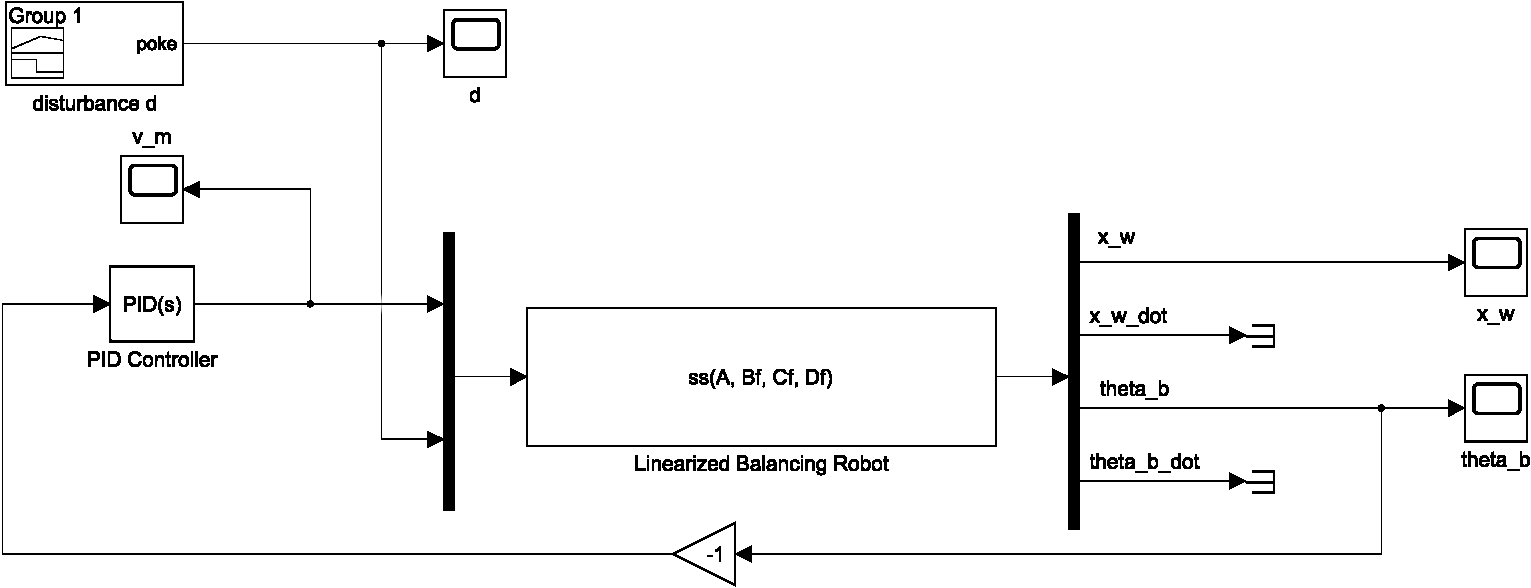
\includegraphics[width=\linewidth]{Images/3.7.1linearizedBot-system.pdf}
    \caption{Simulink scheme for the linearized system, where the
      f-suffix denote the novel matrices.}
    \label{fig:simulink-scheme}
  \end{figure}
\item % plot realizations of ...
  Our realizations of $\theta_b(t)$, $x_w(t)$, $v_m(t)$ and $d(t)$ can
  be seen in Figs.~\ref{fig:lin-theta_b},
  \ref{fig:lin-x_w},
  \ref{fig:lin-v_m},
  \ref{fig:lin-d},
  respectively.
  \begin{figure}
    \centering
    \begin{tabular}{cc}
        \subcaptionbox{Realization of $\theta_b(t)$.\label{fig:lin-theta_b}}{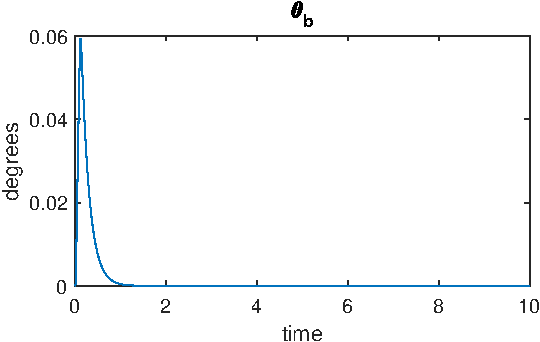
\includegraphics[width=0.5\linewidth]{Images/3.7.1-theta_b.pdf}}&
        \subcaptionbox{Realization of $x_w(t)$.\label{fig:lin-x_w}}{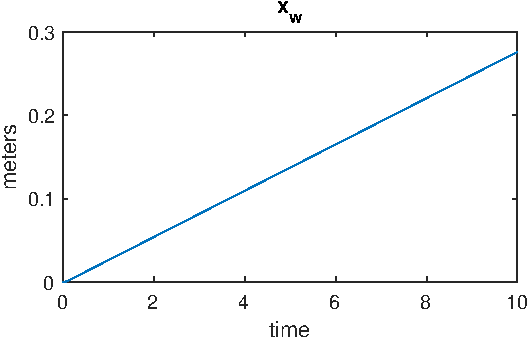
\includegraphics[width=0.5\linewidth]{Images/3.7.1-x_w.pdf}}
      &
        \subcaptionbox{Realization of $v_m(t)$.\label{fig:lin-v_m}}{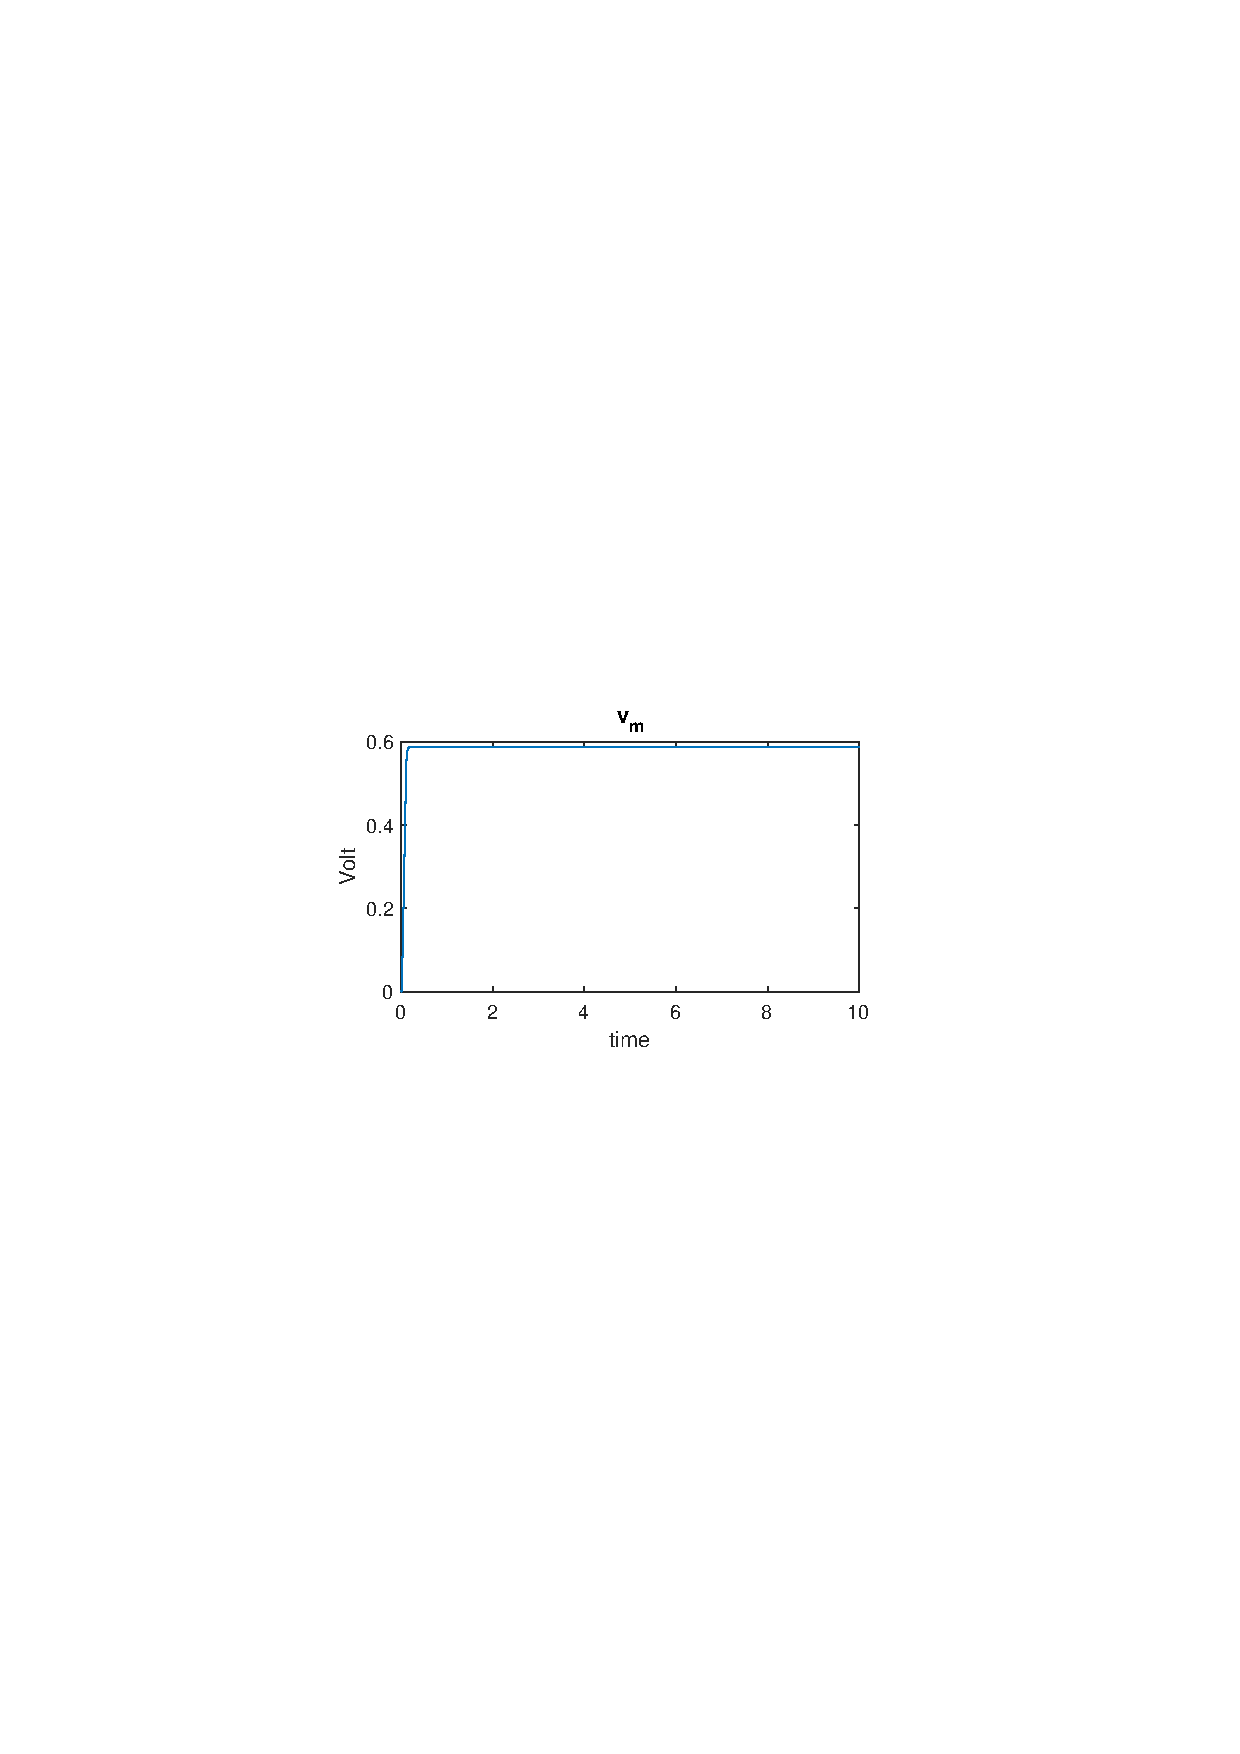
\includegraphics[width=0.5\linewidth]{Images/3.7.1-v_m.pdf}}
      &
        \subcaptionbox{Realization of $d(t)$.\label{fig:lin-d}}{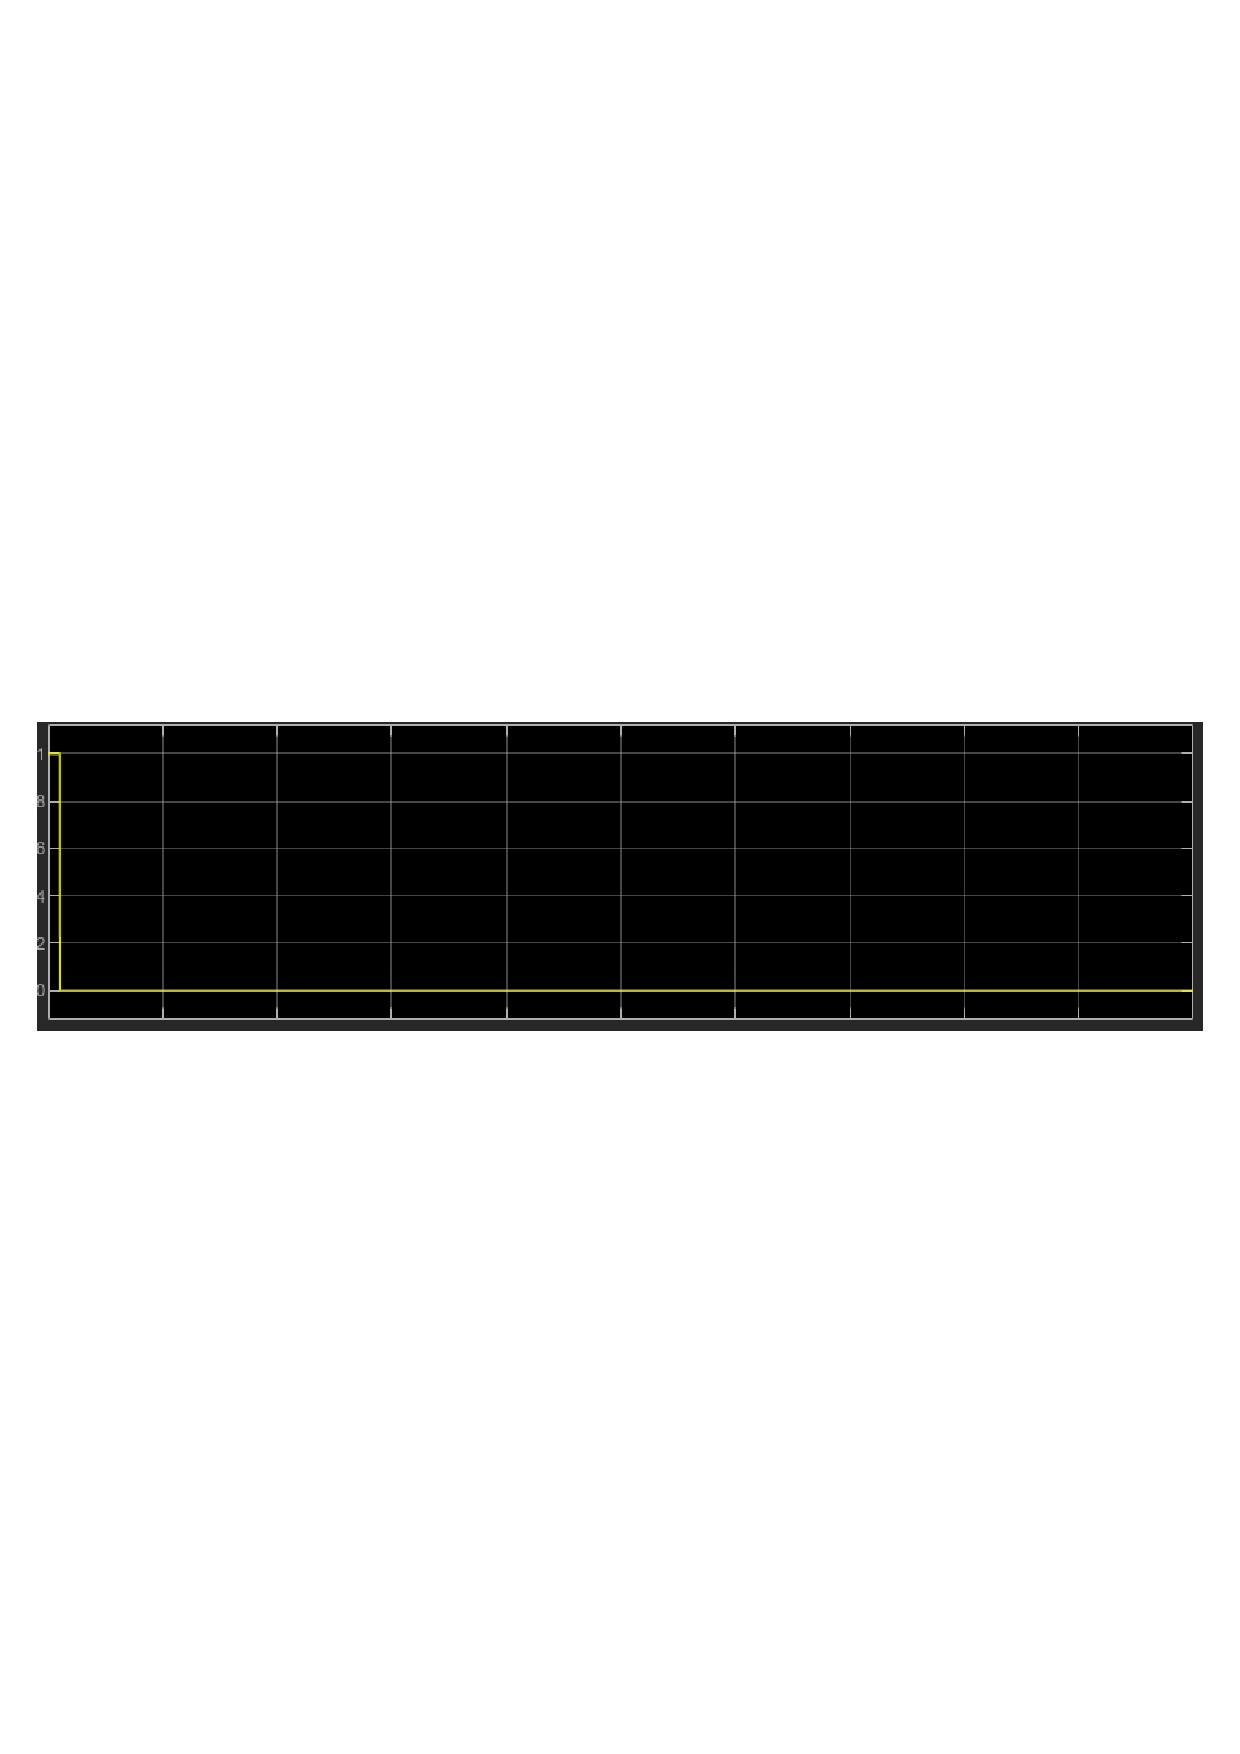
\includegraphics[width=0.5\linewidth]{Images/3.7.1-d.pdf}}
      \\
    \end{tabular}
    \caption{Realizations of the system in Fig.~\ref{fig:simulink-scheme}.}
  \end{figure}
\end{enumerate}

\subsection*{Reporting of Task 3.8.1}
\begin{enumerate}
\item We find the bandwidth of our system via \texttt{gh = plant *
    controller; bandwidth(gh / (1 + gh))} to be
  $\omega_b = 69.8340~\text{rad/s} = 11.1144~\text{Hz}$.
\item We choose our samping time to be
  $25\omega_b \Rightarrow T = 0.0036~\text{s}$.
\item Following the recommendations of §8.3.6, we use a scalar value
  of $25$ so that we may ``[use] discrete equivalents [...] with
  confidence''.
\item
  Our discrete controller, $C(z)$, derived via \texttt{c2d(pid(Kp, Ki,
    Kd, T), T, ’zoh’)}\footnote{We have no idea what value of
    \texttt{Tf} we should pass to \texttt{c2d}, but we assume it has
    some relation to $T$.} is
  \begin{equation}
    C(z) =
    K_p
    + K_i\frac{T_s}{z - 1}
    + K_d\left(
      T_f + \frac{T_s}{z - 1}
    \right)^{-1}
    \text{, where}
    \quad
    \begin{cases}
      K_p = -404 \\
      K_i = -2.26 \times 10^{3} \\
      K_d = -1.33 \\
      T_f = 0.00569 \\
      T_s = T
    \end{cases}
  \end{equation}
\end{enumerate}

\subsection*{Reporting of Task 3.9.1}
\begin{enumerate}
\item % report \bar{d}
  We found that $\bar{d} = 1.54$ for both the discrete and
  continuous case. We presume this to be the expected results on the
  basis that we use $25\omega_b$ as our sampling rate.
\item % plot realizations of cont. and disc.
  Our realizations for $\theta_b(t)$, $v_m(t)$, $\theta^{lin}_b(t)$
  and $v^{lin}_m(t)$ where a continuous controller is used can be seen
  in Figs.~
  \ref{fig:cont-theta_b},
  \ref{fig:cont-v_m},
  \ref{fig:cont-lin-theta_b},
  \ref{fig:cont-lin-v_m},
  respectively.
  \begin{figure}
    \centering
    \begin{tabular}{cc}
        \subcaptionbox{Realization of $\theta_b(t)$.\label{fig:cont-theta_b}}{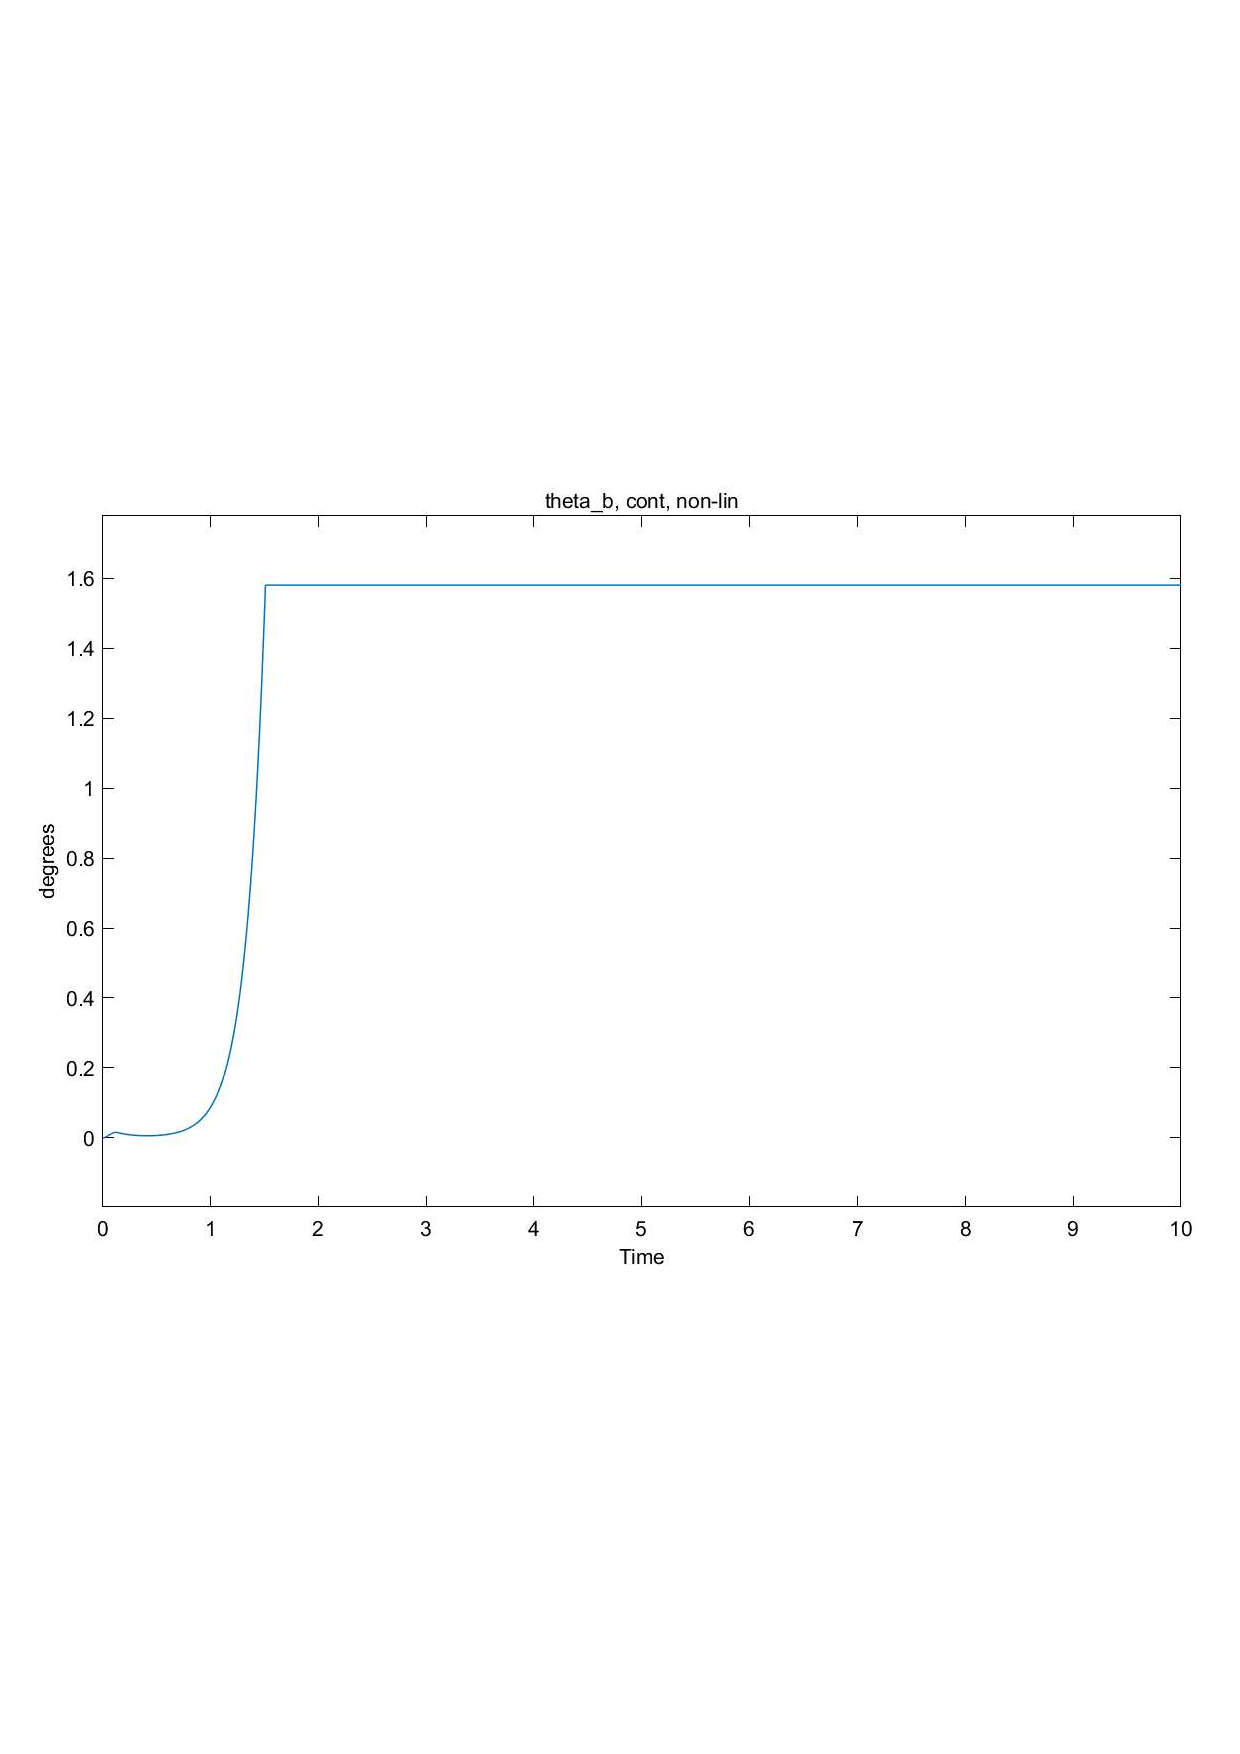
\includegraphics[width=0.5\linewidth]{Images/3.9.1-theta_b-cont-nonlin.pdf}}&
        \subcaptionbox{Realization of $v_m(t)$.\label{fig:cont-v_m}}{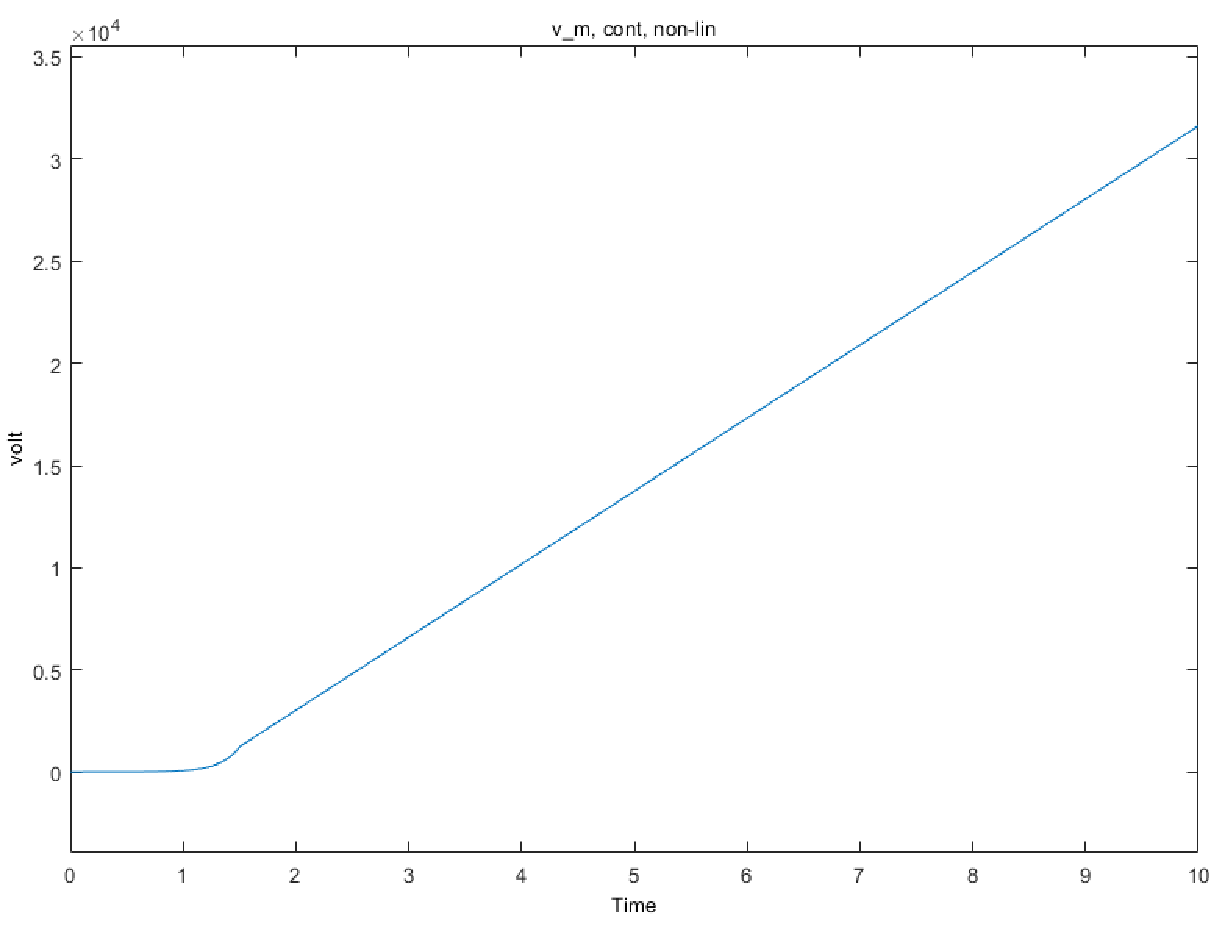
\includegraphics[width=0.5\linewidth]{Images/3.9.1-v_m-cont-nonlin.pdf}}
      &
        \subcaptionbox{Realization of $\theta^{lin}_b(t)$.\label{fig:cont-lin-theta_b}}{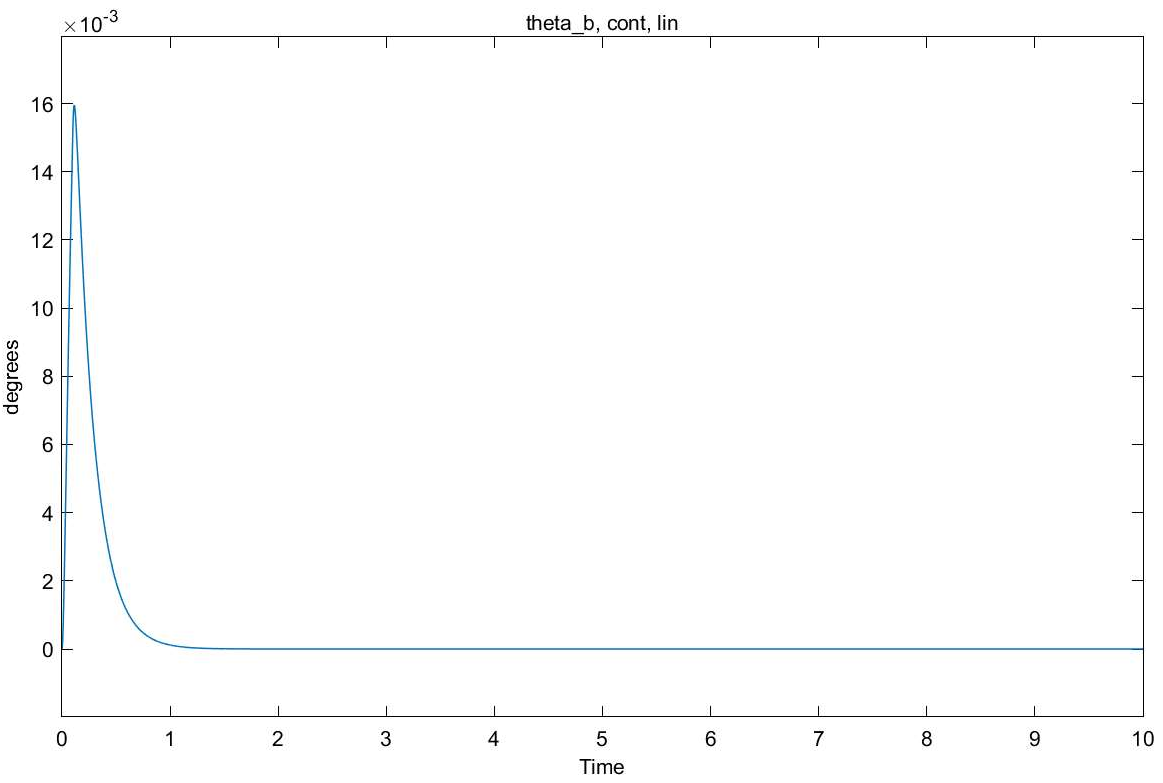
\includegraphics[width=0.5\linewidth]{Images/3.9.1-theta_b-cont-lin.pdf}}
      &
        \subcaptionbox{Realization of $v^{lin}_m(t)$.\label{fig:cont-lin-v_m}}{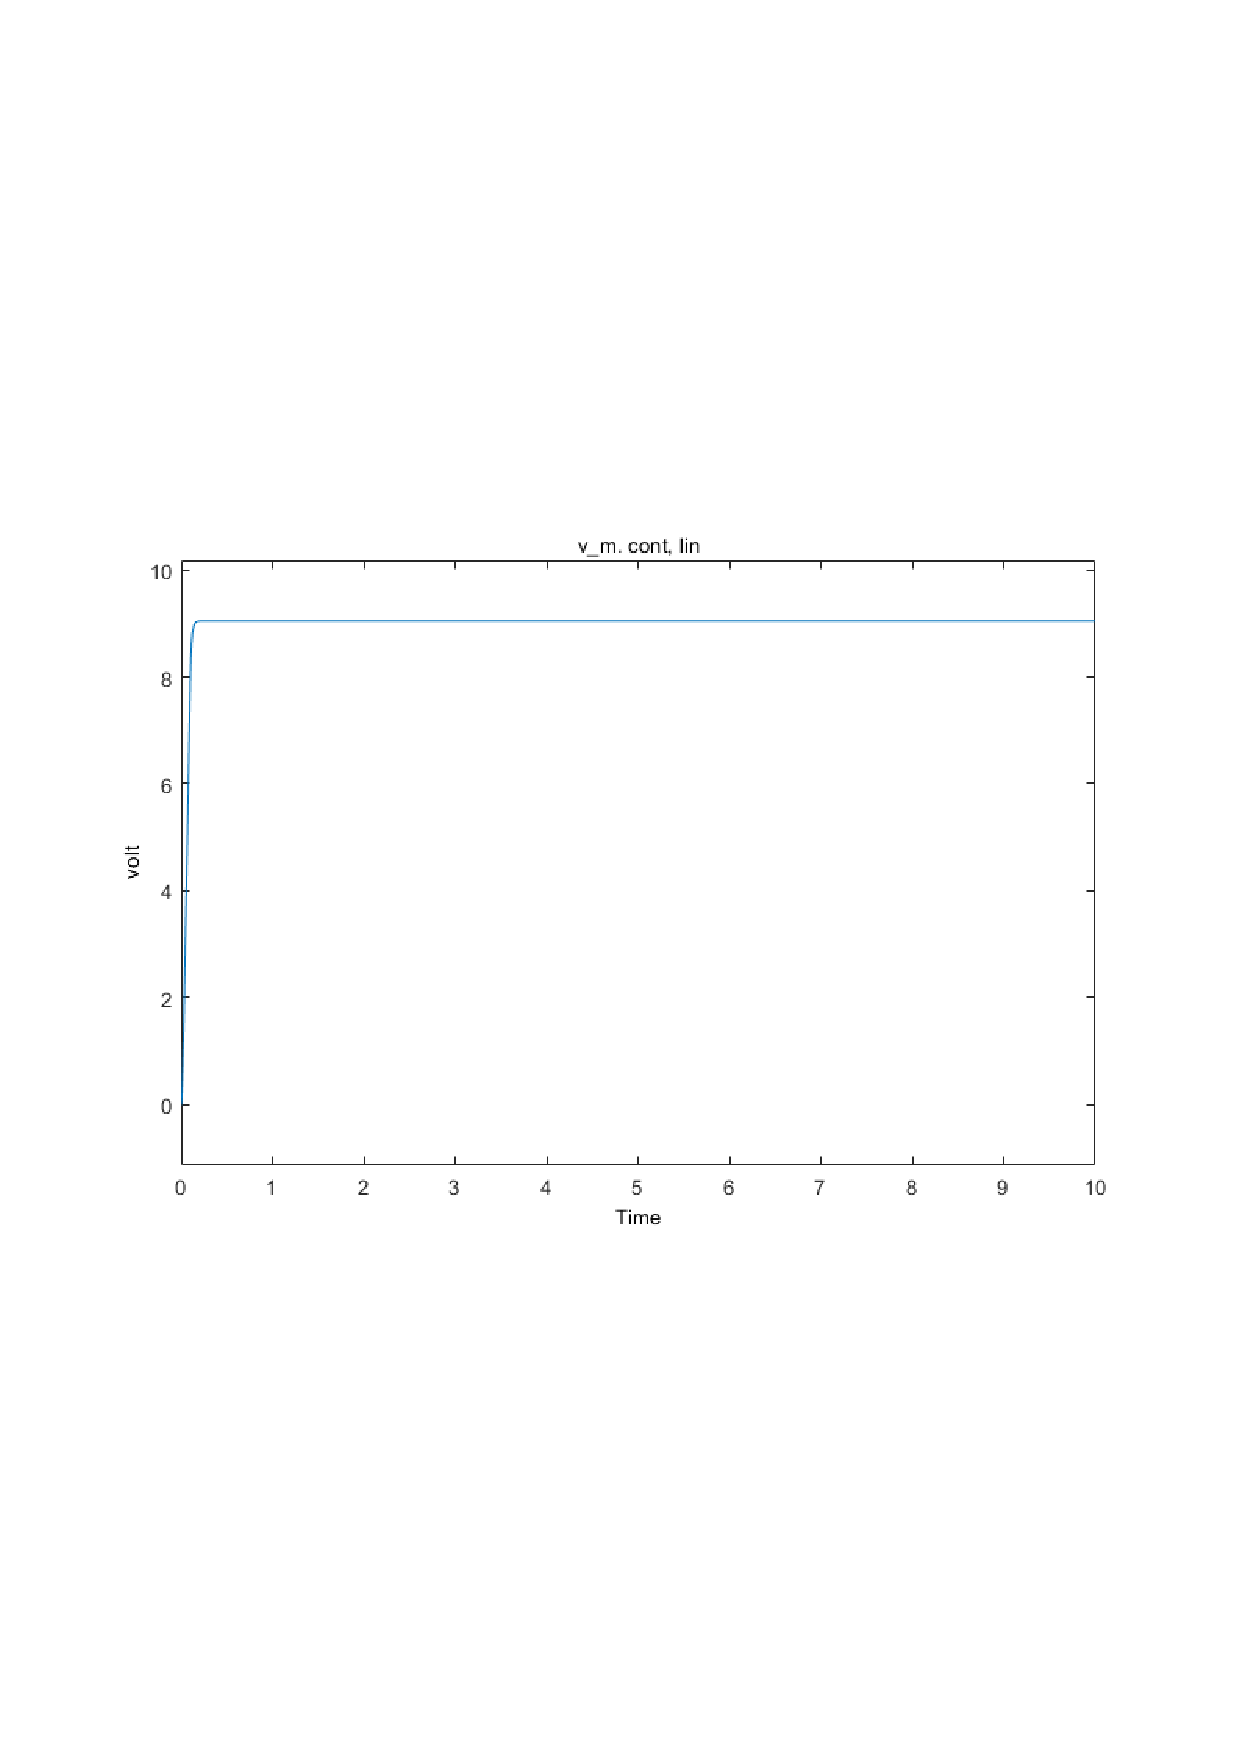
\includegraphics[width=0.5\linewidth]{Images/3.9.1-v_m-cont-lin.pdf}}
      \\
    \end{tabular}
    \caption{Realizations using a continuous controller.}
  \end{figure}

  Our realizations for $\theta_b(k)$, $v_m(k)$, $\theta^{lin}_b(k)$
  and $v^{lin}_m(k)$ where a discrete controller is used can be seen
  in Figs.
  \ref{fig:disc-theta_b},
  \ref{fig:disc-v_m},
  \ref{fig:disc-lin-theta_b},
  \ref{fig:disc-lin-v_m},
  respectively.
    \begin{figure}
    \centering
    \begin{tabular}{cc}
        \subcaptionbox{Realization of $\theta_b(k)$.\label{fig:disc-theta_b}}{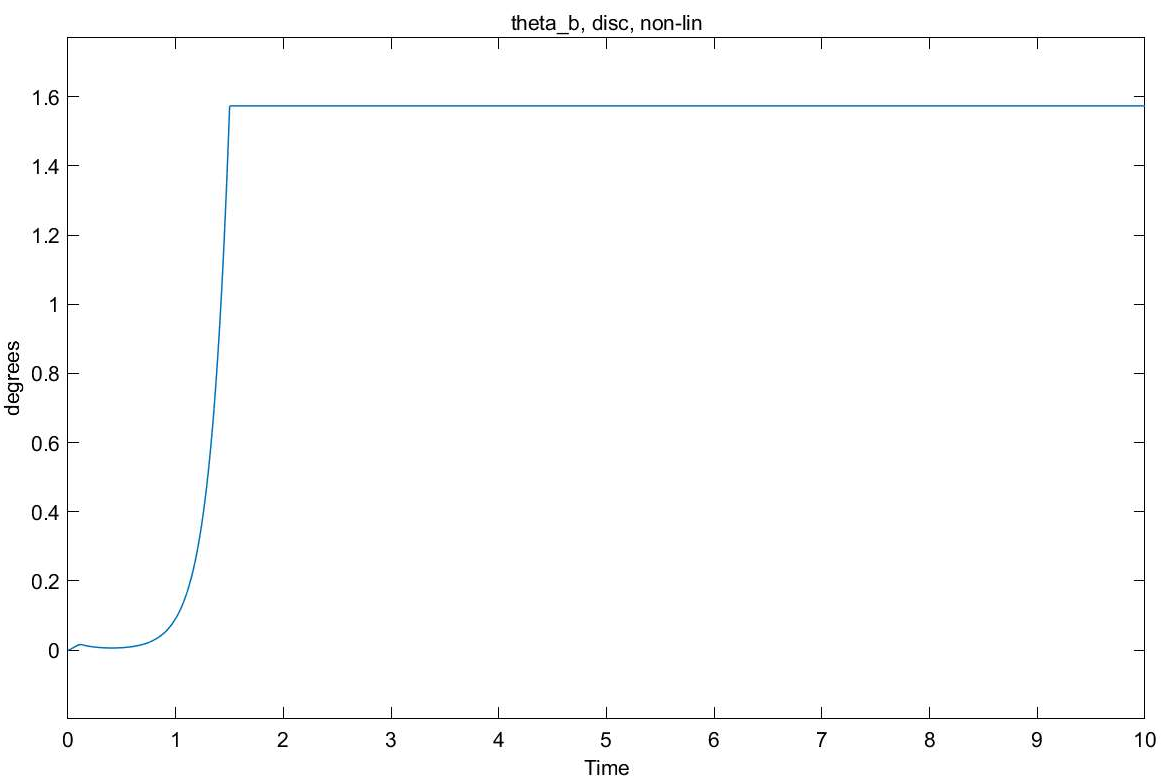
\includegraphics[width=0.5\linewidth]{Images/3.9.1-theta_b-disc-nonlin.pdf}}&
        \subcaptionbox{Realization of $v_m(k)$.\label{fig:disc-v_m}}{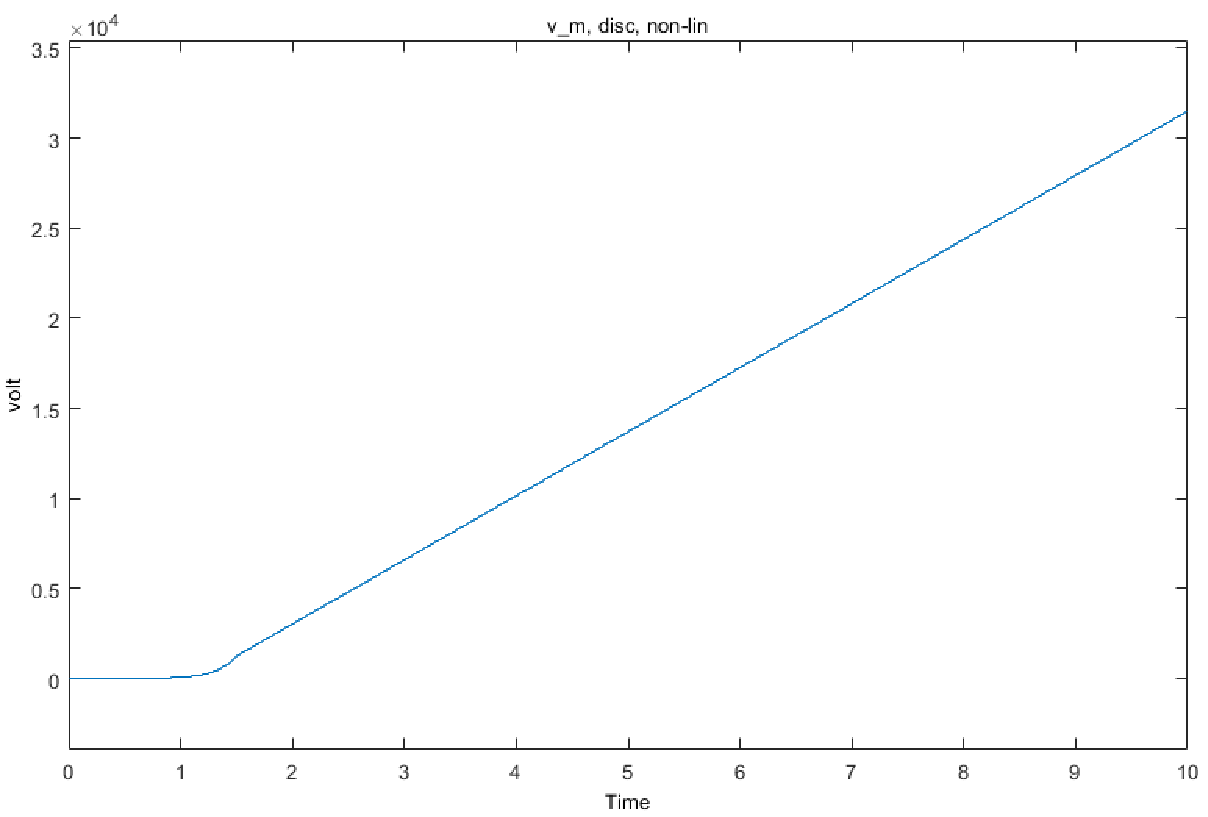
\includegraphics[width=0.5\linewidth]{Images/3.9.1-v_m-disc-nonlin.pdf}}
      &
        \subcaptionbox{Realization of $\theta^{lin}_b(k)$.\label{fig:disc-lin-theta_b}}{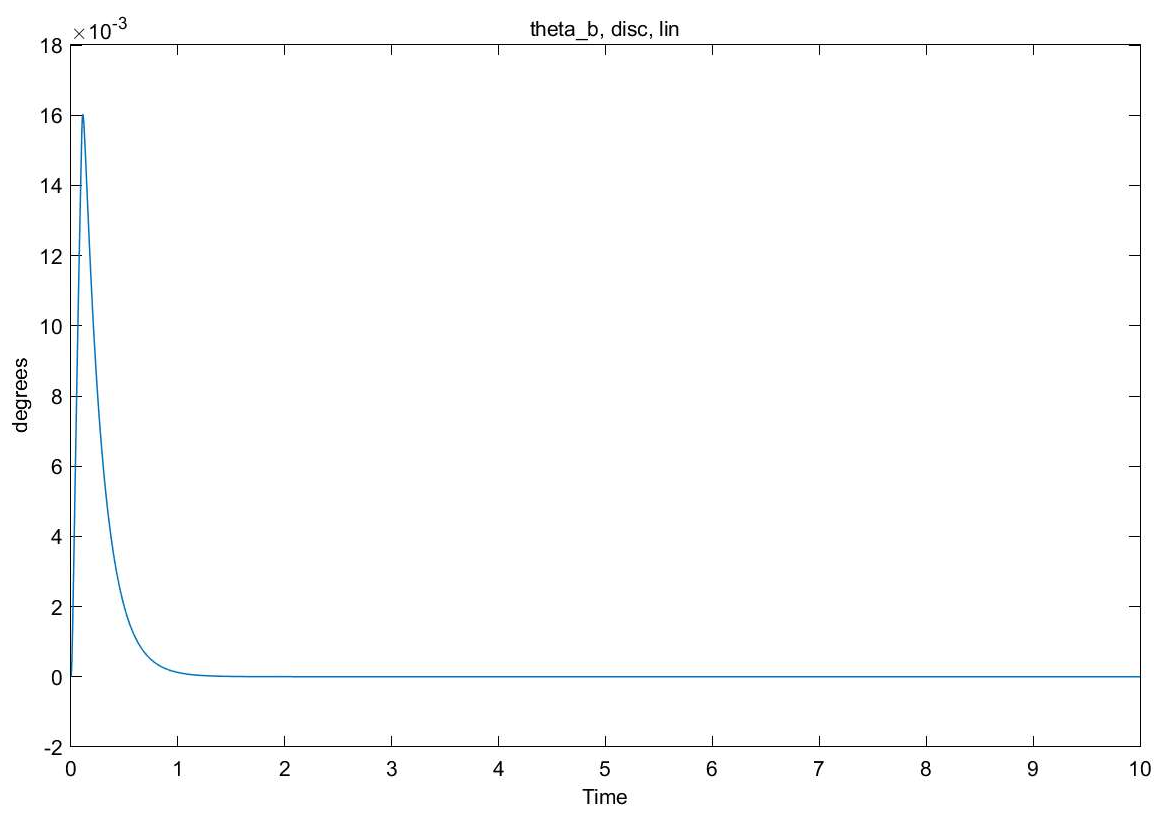
\includegraphics[width=0.5\linewidth]{Images/3.9.1-theta_b-disc-lin.pdf}}
      &
        \subcaptionbox{Realization of $v^{lin}_m(k)$.\label{fig:disc-lin-v_m}}{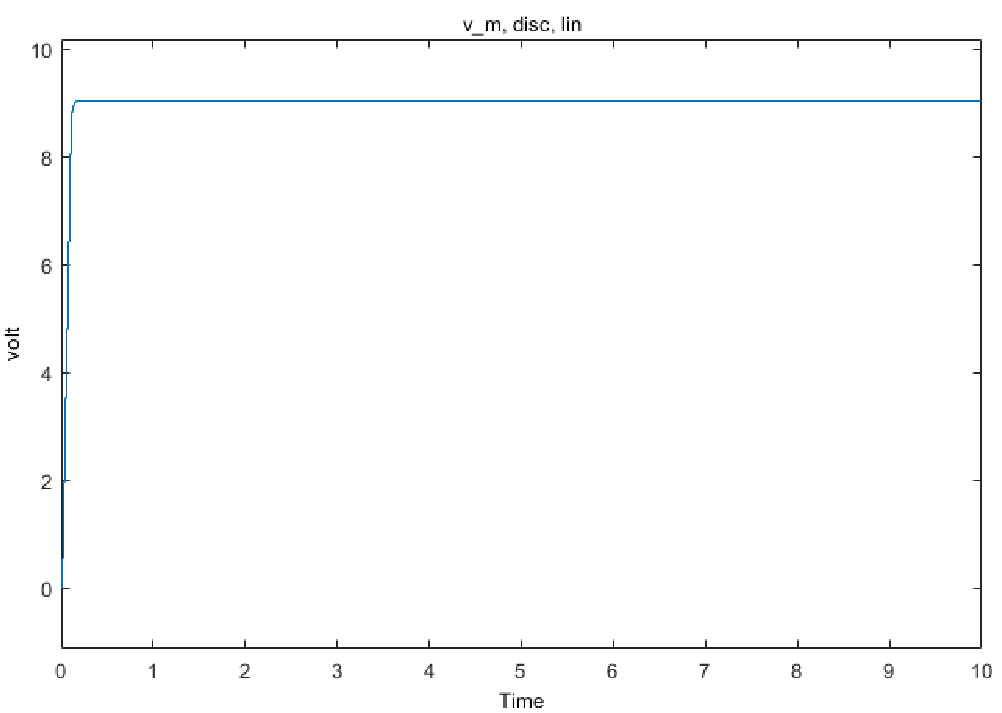
\includegraphics[width=0.5\linewidth]{Images/3.9.1-v_m-disc-lin.pdf}}
      \\
    \end{tabular}
    \caption{Realizations using a discrete controller.}
  \end{figure}
\item % discuss what was understood from these expiremints
  We did not iterate on the \ac{PID} parameters during or after simulating
  because our realizations showed satisfactory results.
\end{enumerate}

\end{document}
